\documentclass{beamer}
	\title{Path Planning for Cable Driven Parallel Robots}
	\author{Hendrik Scheepers de Bruin}
	\institute{École Centrale de Nantes, Università degli Studi di Genova}
	\date{22 July 2019}

    \usepackage{graphicx}
		\graphicspath{{res/img/}}
	\usepackage{multimedia}
	\usepackage{import}

    \usepackage{mathrsfs}
    \usepackage{amsfonts}
    \usepackage{amssymb}
    \usepackage{dsfont}
	\usepackage{amsmath}
    \usepackage{mathtools}
    \usepackage{ifdraft}
    \usepackage[section=subsection, acronyms]{glossaries}
        \makenoidxglossaries{}
        % Dependencies:
%	*	mathrsfs	- for mathscr font
%	*	amsfonts	- for mathfrak and mathbb (upper case) letters
%	*	amssym		- for backepsilon
%	*	dsfont		- for mathds
\newglossary*{notation}{Notation}

% ==============================================================================
% Scalar
% ==============================================================================
	\newglossaryentry{not:scalar}
	{%
		name=\ensuremath{m},
		description=a scalar,
		type=notation
	}
	\glsadd{not:scalar}

% ==============================================================================
% Vector
% ==============================================================================
	\renewcommand{\vec}[1]{\ensuremath{\boldsymbol{#1}}}
	\newglossaryentry{not:vec}
	{%
		name=\vec{m}\ifdraft{: \textbackslash{} vec}{},
		description=a vector,
		type=notation
	}
	\glsadd{not:vec}

% ==============================================================================
% Projection
% ==============================================================================
	\newcommand{\project}[2]{\ensuremath{{}^{#2}\!{#1}}}
	\newglossaryentry{not:project}
	{%
		name=\project{\vec{m}}{n}\ifdraft{: \textbackslash{} project\{to\}}{},,
		description=projection of vector \vec{m} in frame $n$,
		type=notation
	}
	\glsadd{not:project}

% ==============================================================================
% Skew Matrix
% ==============================================================================
	\newcommand{\skewmat}[1]{\ensuremath{\widehat{#1}}}
	%\newcommand{\skewmat}[1]{\ensuremath{\left[{#1}\right]_{\mathrm{X}}}}
	\newglossaryentry{not:skewmat}
	{%
		name=\skewmat{\vec{m}}\ifdraft{: \textbackslash{} skew}{},
		description=the skew matrix associated with the vector \vec{m},
		type=notation
	}
	\glsadd{not:skewmat}

% ==============================================================================
% Matrix
% ==============================================================================
	\newcommand{\mat}[1]{\ensuremath{\boldsymbol{\mathrm{#1}}}}
	\newglossaryentry{not:mat}
	{%
		name=\mat{M}\ifdraft{: \textbackslash{} mat}{},
		description=a matrix,
		type=notation
	}
	\glsadd{not:mat}

% ==============================================================================
% Pseudo Inverse
% ==============================================================================
	\newcommand{\pseudoinv}[1]{\ensuremath{{#1}^{+}}}
	\newglossaryentry{not:pseudoinv}
	{%
		name=\pseudoinv{\mat{M}}\ifdraft{: \textbackslash{} pseudoinv}{},
		description=the pseudo inverse of matrix \mat{M},
		type=notation
	}
	\glsadd{not:pseudoinv}

% ==============================================================================
% Vector Space
% ==============================================================================
	\newcommand{\vecspace}[1]{\ensuremath{\mathscr{#1}}}
	\newglossaryentry{not:vecspace}
	{%
		name=\vecspace{M}\ifdraft{: \textbackslash{} vecspace}{},
		description=a vector space,
		type=notation
	}
	\glsadd{not:vecspace}

% ==============================================================================
% Set
% ==============================================================================
	\newcommand{\set}[1]{\ensuremath{\mathcal{#1}}}
	\newglossaryentry{not:set}
	{%
		name=\set{M}\ifdraft{: \textbackslash{} set}{},
		description=a set,
		type=notation
	}
	\glsadd{not:set}

% ==============================================================================
% Function
% ==============================================================================
	\newcommand{\func}[1]{\ensuremath{\mathrm{#1}}}
	\newglossaryentry{not:func}
	{%
		name=\func{m}\ifdraft{: \textbackslash{} func}{},
		description=a function,
		type=notation
	}
	\glsadd{not:func}

% ==============================================================================
% Vector Function
% ==============================================================================
	\newcommand{\vecfunc}[1]{\ensuremath{\boldsymbol{\mathrm{#1}}}}
	\newglossaryentry{not:vecfunc}
	{%
		name=\vecfunc{m}\ifdraft{: \textbackslash{} vecfunc}{},
		description=a vector function,
		type=notation
	}
	\glsadd{not:vecfunc}

% ==============================================================================
% Estimate
% ==============================================================================
	\newcommand{\estimate}[1]{\ensuremath{\widetilde{#1}}}
	\newglossaryentry{not:estimate}
	{%
		name=\estimate{m}\ifdraft{: \textbackslash{} estimate}{},
		description=an estimate of the quantity $m$,
		type=notation
	}
	\glsadd{not:estimate}

% ==============================================================================
% nth Time Derivative
% ==============================================================================
	\newcommand{\tdern}[2]{\ensuremath{{#1}^{(#2)}}}
	\newglossaryentry{not:tdern}
	{%
		name=\tdern{m}{n}\ifdraft{: \textbackslash{} tdern}{},
		description=the nth time derivative of quantity $m$,
		type=notation
	}
	\glsadd{not:tdern}

% ==============================================================================
% Desired Value
% ==============================================================================
	\newcommand{\desired}[1]{\ensuremath{{#1}^{*}}}
	\newglossaryentry{not:desired}
	{%
		name=\desired{m}\ifdraft{: \textbackslash{} desired}{},
		description=the desired value of $m$,
		type=notation
	}
	\glsadd{not:desired}

% ==============================================================================
% Such That
% ==============================================================================
	\newglossaryentry{not:suchthat}
	{%
		name={\ensuremath{\backepsilon}},
		description=such that,
		type=notation
	}
	\newcommand{\suchthat}{\gls{not:suchthat}}

        \newglossary*{symbol}{Symbols}
% ==============================================================================
% Sample
% ==============================================================================
	\newglossaryentry{sym:sample}
	{%
		name=\ensuremath{\sigma},
		sort=s,
		description=sample,
		type=symbol
	}
	\newcommand{\sample}{\gls{sym:sample}}

% ==============================================================================
% Distance
% ==============================================================================
	\newglossaryentry{sym:distance}
	{%
		name=\ensuremath{d},
		sort=h,
		description=distance,
		type=symbol
	}
	\newcommand{\distance}{\gls{sym:distance}}

% ==============================================================================
% Quaternion
% ==============================================================================
	\newglossaryentry{sym:quaternion}
	{%
		name=\ensuremath{\vec{h}},
		sort=h,
		description=quaternion,
		type=symbol
	}
	\newcommand{\quaternion}{\gls{sym:quaternion}}

% ==============================================================================
% Queue
% ==============================================================================
	\newglossaryentry{sym:queue}
	{%
		name=\ensuremath{\code{q}},
		sort=q,
		description=queue,
		type=symbol
	}
	\newcommand{\queue}{\gls{sym:queue}}

% ==============================================================================
% Torque
% ==============================================================================
	\newglossaryentry{sym:torque}
	{%
		name=\ensuremath{\vec{\tau}},
		sort=t,
		description=torque,
		type=symbol
	}
	\newcommand{\torque}{\gls{sym:torque}}

% ==============================================================================
% Gain
% ==============================================================================
	\newglossaryentry{sym:gain}
	{%
		name={\ensuremath{\lambda}},
		sort=l,
		description=A tunable gain,
		type=symbol
	}
	\newcommand{\gain}{\gls{sym:gain}}

% ==============================================================================
% Point
% ==============================================================================
	\newglossaryentry{sym:point}
	{%
		name={\ensuremath{\vec{p}}},
		sort=p,
		description=A point in space,
		type=symbol
	}
	\newcommand{\point}{\gls{sym:point}}

% ==============================================================================
% Set of Points
% ==============================================================================
	\newglossaryentry{sym:setofpoints}
	{%
		name={\ensuremath{\set{P}}},
		sort=p,
		description=A set of points in space,
		type=symbol
	}
	\newcommand{\setofpoints}{\gls{sym:setofpoints}}

% ==============================================================================
% Trajectory
% ==============================================================================
	\newglossaryentry{sym:traj}
	{%
		name={\ensuremath{\vec{s}}},
		sort=s,
		description=A trajectory in space,
		type=symbol
	}
	\newcommand{\traj}{\gls{sym:traj}}

% ==============================================================================
% Path
% ==============================================================================
	\newcommand{\pathsym}{\traj}


% ==============================================================================
% Time
% ==============================================================================
	\newglossaryentry{sym:time}
	{%
		name={\ensuremath{t}},
		sort=t,
		description=time,
		type=symbol
	}
	\newcommand{\timesym}{\gls{sym:time}}

% ==============================================================================
% Time Normalised
% ==============================================================================
	\newglossaryentry{sym:timenorm}
	{%
		name={\ensuremath{\tau}},
		sort=t,
		description=normalised time \ensuremath{\tau \in [0, 1]},
		type=symbol
	}
	\newcommand{\timenorm}{\gls{sym:timenorm}}

% ==============================================================================
% Set of Time Instants
% ==============================================================================
	\newglossaryentry{sym:setoftimeinstants}
	{%
		name={\ensuremath{\set{T}}},
		sort=t,
		description=A set of time instants,
		type=symbol
	}
	\newcommand{\setoftimeinstants}{\gls{sym:setoftimeinstants}}

% ==============================================================================
% Period
% ==============================================================================
	\newglossaryentry{sym:period}
	{%
		name={\ensuremath{T}},
		sort=t,
		description=period,
		type=symbol
	}
	\newcommand{\period}{\gls{sym:period}}

% ==============================================================================
% Tolerance
% ==============================================================================
	\newglossaryentry{sym:tolerance}
	{%
		name={\ensuremath{\epsilon}},
		sort=e,
		description=Tolerance,
		type=symbol
	}
	\newcommand{\tol}{\gls{sym:tolerance}}

% ==============================================================================
% Geometric Model
% ==============================================================================
	\newglossaryentry{sym:geometricmodel}
	{%
		name={\ensuremath{\vecfunc{g}}},
		sort=G,
		description=Geometric Model,
		type=symbol
	}
	\newcommand{\geometricmodel}{\gls{sym:geometricmodel}}

% ==============================================================================
% Inverse Geometric Model
% ==============================================================================
	\newglossaryentry{sym:invgeometricmodel}
	{%
		name={\ensuremath{{\vecfunc{g}^{-1}}}},
		sort=G,
		description=Inverse Geometric Model,
		type=symbol
	}
	\newcommand{\invgeometricmodel}{\gls{sym:invgeometricmodel}}
% ==============================================================================
% Kinematic Model
% ==============================================================================
	\newglossaryentry{sym:kinematicmodel}
	{%
		name={\ensuremath{\vecfunc{k}}},
		sort=K,
		description=Kinematic Model,
		type=symbol
	}
	\newcommand{\kinematicmodel}{\gls{sym:kinematicmodel}}

% ==============================================================================
% Inverse Kinematic Model
% ==============================================================================
	\newglossaryentry{sym:invkinematicmodel}
	{%
		name={\ensuremath{{\vecfunc{k}^{-1}}}},
		sort=K,
		description=Inverse Kinematic Model,
		type=symbol
	}
	\newcommand{\invkinematicmodel}{\gls{sym:invkinematicmodel}}
% ==============================================================================
% Dynamic Model
% ==============================================================================
	\newglossaryentry{sym:dynamicmodel}
	{%
		name={\ensuremath{\vecfunc{d}}},
		sort=d,
		description=Dynamic Model,
		type=symbol
	}
	\newcommand{\dynamicmodel}{\gls{sym:dynamicmodel}}

% ==============================================================================
% Inverse Dynamic Model
% ==============================================================================
	\newglossaryentry{sym:invdynamicmodel}
	{%
		name={\ensuremath{{\vecfunc{d}^{-1}}}},
		sort=d,
		description=Inverse Dynamic Model,
		type=symbol
	}
	\newcommand{\invdynamicmodel}{\gls{sym:invdynamicmodel}}

% ==============================================================================
% Constraint
% ==============================================================================
	\newglossaryentry{sym:constraint}
	{%
		%name=\protect\reflectbox{\ensuremath{\mathds{C}}},
		%name=\protect\reflectbox{\ensuremath{\mat{C}}},
		name=\ensuremath{c},
		sort=c,
		description=constraint,
		type=symbol
	}
	\newcommand{\constraint}{\gls{sym:constraint}}

% ==============================================================================
% Set of Constraints
% ==============================================================================
	\newglossaryentry{sym:setofconstraints}
	{%
		%name=\protect\reflectbox{\ensuremath{\set{C}}},
		%name=\protect\reflectbox{\ensuremath{\mat{C}}},
		name=\ensuremath{\set{C}},
		sort=c,
		description=set of constraints,
		type=symbol
	}
	\newcommand{\setofconstraints}{\gls{sym:setofconstraints}}

% ==============================================================================
% Configuration
% ==============================================================================
	\newglossaryentry{sym:configuration}
	{%
		name=\ensuremath{q},
		sort=q,
		description=Configuration,
		type=symbol
	}
	\newcommand{\configuration}{\gls{sym:configuration}}

%TODO indexes
% ==============================================================================
% Index i
% ==============================================================================
	\newglossaryentry{sym:indexi}
	{%
		name=\ensuremath{i},
		sort=i,
		description=an index,
		type=symbol
	}
	\newcommand{\indexi}{\gls{sym:indexi}}
% ==============================================================================
% Index j
% ==============================================================================
	\newglossaryentry{sym:indexj}
	{%
		name=\ensuremath{j},
		sort=j,
		description=an index,
		type=symbol
	}
	\newcommand{\indexj}{\gls{sym:indexj}}

% ==============================================================================
% Index k
% ==============================================================================
	\newglossaryentry{sym:indexk}
	{%
		name=\ensuremath{k},
		sort=k,
		description=an index,
		type=symbol
	}
	\newcommand{\indexk}{\gls{sym:indexk}}

% ==============================================================================
% State
% ==============================================================================
	\newglossaryentry{sym:state}
	{%
		name=\ensuremath{\vec{x}},
		sort=x,
		description=the state  of the robot,
		type=symbol
	}
	\newcommand{\state}{\gls{sym:state}}

% ==============================================================================
% State Space
% ==============================================================================
	\newglossaryentry{sym:statespace}
	{%
		name=\ensuremath{\vecspace{X}},
		sort=x,
		description=the state space of the robot,
		type=symbol
	}
	\newcommand{\statespace}{\gls{sym:statespace}}

% ==============================================================================
% Inverse Action
% ==============================================================================
	\newglossaryentry{sym:invaction}
	{%
		name=\ensuremath{\vec{u}^{-1}},
		sort=u,
		description=the inverse action  of the robot,
		type=symbol
	}
	\newcommand{\invaction}{\gls{sym:invaction}}
% ==============================================================================
% Action
% ==============================================================================
	\newglossaryentry{sym:action}
	{%
		name=\ensuremath{\vec{u}},
		sort=u,
		description=the action  of the robot,
		type=symbol
	}
	\newcommand{\action}{\gls{sym:action}}

% ==============================================================================
% Action Space
% ==============================================================================
	\newglossaryentry{sym:actionspace}
	{%
		name=\ensuremath{\vecspace{U}},
		sort=u,
		description=the action space of the robot,
		type=symbol
	}
	\newcommand{\actionspace}{\gls{sym:actionspace}}

% ==============================================================================
% Inverse Action Space
% ==============================================================================
	\newglossaryentry{sym:invactionspace}
	{%
		name=\ensuremath{\vecspace{U}^{-1}},
		sort=u,
		description=the inverse action space of the robot,
		type=symbol
	}
	\newcommand{\invactionspace}{\gls{sym:invactionspace}}

% ==============================================================================
% Configuration Space
% ==============================================================================
	\newglossaryentry{sym:configurationspace}
	{%
		name=\ensuremath{\vecspace{C}},
		sort=c,
		description=the configuration space of the robot,
		type=symbol
	}
	\newcommand{\configurationspace}{\gls{sym:configurationspace}}
% ==============================================================================
% World Space
% ==============================================================================
	\newglossaryentry{sym:worldspace}
	{%
		name=\ensuremath{\vecspace{W}},
		sort=w,
		description=the world inhabited by the robot,
		type=symbol
	}
	\newcommand{\world}{\gls{sym:worldspace}}

%%TODO Polynomials
% ==============================================================================
% B-Spline
% ==============================================================================
	\newglossaryentry{sym:bspline}
	{%
		name=\ensuremath{\vec{B}},
		sort=b,
		description=B-spline basis function,
		type=symbol
	}
	\newcommand{\bspline}{\gls{sym:bspline}}
% ==============================================================================
% knot
% ==============================================================================
	\newglossaryentry{sym:knot}
	{%
		name=\ensuremath{\vec{k}},
		sort=k,
		description=B-spline knot vector,
		type=symbol
	}
	\newcommand{\knot}{\gls{sym:knot}}
% ==============================================================================
% Coefficient
% ==============================================================================
	\newglossaryentry{sym:polynomial}
	{%
		name=\ensuremath{\func{p}},
		sort=p,
		description=a polynomial function,
		type=symbol
	}
	\newcommand{\polynomial}{\gls{sym:polynomial}}

% ==============================================================================
% Coefficient
% ==============================================================================
	\newglossaryentry{sym:coefficient}
	{%
		name=\ensuremath{a},
		sort=a,
		description=Polynomial Coefficient,
		type=symbol
	}
	\newcommand{\coefficient}{\gls{sym:coefficient}}

% ==============================================================================
% Coefficient
% ==============================================================================
	\newglossaryentry{sym:coefficientb}
	{%
		name=\ensuremath{b},
		sort=b,
		description=Polynomial Coefficient,
		type=symbol
	}
	\newcommand{\coefficientb}{\gls{sym:coefficientb}}

% ==============================================================================
% Polynomial Degree
% ==============================================================================
	\newglossaryentry{sym:poldeg}
	{%
		name=\ensuremath{n},
		sort=n,
		description=Polynomial Degree,
		type=symbol
	}
	\newcommand{\poldeg}{\gls{sym:poldeg}}

% ==============================================================================
% Polynomial Degree
% ==============================================================================
	\newglossaryentry{sym:relweight}
	{%
		name=\ensuremath{\mu},
		sort=m,
		description=relative weight of a factor \ensuremath{\mu \in [0, 1]},
		type=symbol
	}
	\newcommand{\relweight}{\gls{sym:relweight}}

% ==============================================================================
% Half Space Primitive
% ==============================================================================
	\newglossaryentry{sym:halfspaceprimitive}
	{%
		name=\ensuremath{\set{H}},
		sort=h,
		description=a half space primitive,
		type=symbol
	}
	\newcommand{\halfspaceprimitive}{\gls{sym:halfspaceprimitive}}

% ==============================================================================
% Transform function
% ==============================================================================
	\newglossaryentry{sym:transform}
	{%
		name=\ensuremath{\func{h}},
		sort=h,
		description=a transform function,
		type=symbol
	}
	\newcommand{\transform}{\gls{sym:transform}}
% ==============================================================================
% Robot DOF
% ==============================================================================
	\newglossaryentry{sym:robotdof}
	{%
		name=\ensuremath{m},
		sort=m,
		description=robot degrees of freedom,
		type=symbol
	}
	\newcommand{\robotdof}{\gls{sym:robotdof}}

% ==============================================================================
% Robot
% ==============================================================================
	\newglossaryentry{sym:robot}
	{%
		name=\ensuremath{\set{A}},
		sort=a,
		description=a robot,
		type=symbol
	}
	\newcommand{\robot}{\gls{sym:robot}}

% ==============================================================================
% Point in Robot
% ==============================================================================
	\newglossaryentry{sym:pointinrobot}
	{%
		name=\ensuremath{\vec{a}},
		sort=a,
		description=a point in a robot,
		type=symbol
	}
	\newcommand{\pointinrobot}{\gls{sym:pointinrobot}}

% ==============================================================================
% Obstacle
% ==============================================================================
	\newglossaryentry{sym:obstacle}
	{%
		name=\ensuremath{\set{O}},
		sort=o,
		description=an obstacle,
		type=symbol
	}
	\newcommand{\obstacle}{\gls{sym:obstacle}}

% ==============================================================================
% Obstacle
% ==============================================================================
	\newglossaryentry{sym:logicalpredicate}
	{%
		name=\ensuremath{\func{\phi}},
		sort=f,
		description=an logical predicate,
		type=symbol
	}
	\newcommand{\logicalpredicate}{\gls{sym:logicalpredicate}}

% ==============================================================================
% True
% ==============================================================================
	\newglossaryentry{sym:true}
	{%
		name=\ensuremath{\top},
		sort=t,
		description=true,
		type=symbol
	}
	\newcommand{\true}{\gls{sym:true}}

% ==============================================================================
% False
% ==============================================================================
	\newglossaryentry{sym:false}
	{%
		name=\ensuremath{\bot},
		sort=t,
		description=false,
		type=symbol
	}
	\newcommand{\false}{\gls{sym:false}}

% ==============================================================================
% Swath
% ==============================================================================
	\newglossaryentry{sym:swath}
	{%
		name=\ensuremath{\set{S}},
		sort=s,
		description=the set of points reached by a topological graph,
		type=symbol
	}
	\newcommand{\swath}{\gls{sym:swath}}

% ==============================================================================
% Graph
% ==============================================================================
	\newglossaryentry{sym:topologicalgraph}
	{%
		name=\ensuremath{\set{G}},
		sort=g,
		description=topological graph,
		type=symbol
	}
	\newcommand{\topologicalgraph}{\gls{sym:topologicalgraph}}

% ==============================================================================
% Edge
% ==============================================================================
	\newglossaryentry{sym:edge}
	{%
		name=\ensuremath{\vec{e}},
		sort=e,
		description=edge of a graph,
		type=symbol
	}
	\newcommand{\edge}{\gls{sym:edge}}

% ==============================================================================
% Vertex
% ==============================================================================
	\newglossaryentry{sym:vertex}
	{%
		name=\ensuremath{\vec{v}},
		sort=e,
		description=vertex of a graph,
		type=symbol
	}
	\newcommand{\vertex}{\gls{sym:vertex}}

        \newacronym{sat}{SAT}{Separting Axis Theorem}
\newacronym{dof}{dof}{Degree of Freedom}
\newacronym{cdpr}{CDPR}{Cable-Driven Parallel Robot}
\newacronym{dgm}{DGM}{Direct Geometric Model}
\newacronym{igm}{IGM}{Indirect Geometric Model}
\newacronym{dkm}{DKM}{Direct Kinematic Model}
\newacronym{ikm}{IKM}{Indirect Kineamtic Model}
\newacronym{ddm}{DDM}{Direct Dynamic Model}
\newacronym{idm}{IDM}{Inverse Dynamic Model}
\newacronym{fifo}{FIFO}{First-In-First-Out}
\newacronym{lifo}{LIFO}{Last-In-First-Out}
\newacronym{rdt}{RDT}{Rapidly Exploring Dense Tree}
\newacronym{rrt}{RRT}{Rapidly Exploring Random Tree}
\newacronym{cad}{CAD}{Computer Aided Design}
\newacronym{csp}{CSP}{Constraint Satisfaction Problem}

\newacronym{irpm}{IRPM}{Incompletely Restrained Positioning Mechanism}
\newacronym{crpm}{CRPM}{Completely Restrained Positioning Mechanism}
\newacronym{rrpm}{RRPM}{Redundantly Restrained Positioning Mechanism}

        \newglossary*{defs}{Glossary}

\newglossaryentry{jolt}
{%
	name=jolt,
	description=The first time derivative of acceleration (in some texts referred to as ``jerk''),
	type=defs
}

\newglossaryentry{jounce}
{%
	name=jounce,
	description=The second time derivative of acceleration,
	type=defs
}

        \newglossary*{subscript}{Subscripts}

% ==============================================================================
% Final
% ==============================================================================
	\newglossaryentry{sub:final}
	{%
		name={\ensuremath{\mathrm{F}}},
		sort=f,
		description=Final,
		type=subscript
	}
	\newcommand{\final}{\gls{sub:final}}

% ==============================================================================
% Goal
% ==============================================================================
	\newglossaryentry{sub:goal}
	{%
		name={\ensuremath{\mathrm{G}}},
		sort=g,
		description=goal,
		type=subscript
	}
	\newcommand{\goal}{\gls{sub:goal}}

% ==============================================================================
% Initial
% ==============================================================================
	\newglossaryentry{sub:initial}
	{%
		name={\ensuremath{\mathrm{I}}},
		sort=i,
		description=initial,
		type=subscript
	}
	\newcommand{\initial}{\gls{sub:initial}}

% ==============================================================================
% Obstacle Region
% ==============================================================================
	\newglossaryentry{sub:obstacleregion}
	{%
		name={\ensuremath{\mathrm{obs}}},
		sort=obs,
		description=obstacle region,
		type=subscript
	}
	\newcommand{\obstacleregion}{\gls{sub:obstacleregion}}

% ==============================================================================
% Free Region
% ==============================================================================
	\newglossaryentry{sub:freeregion}
	{%
		name={\ensuremath{\mathrm{free}}},
		sort=obs,
		description=free region,
		type=subscript
	}
	\newcommand{\freeregion}{\gls{sub:freeregion}}


	\let\beameraction\action%

	\usepackage{caption}

	\usepackage[citestyle=numeric,bibstyle=numeric]{biblatex}
		\addbibresource{bib/cdpr.bib}
		\addbibresource{bib/path_planning.bib}
		\addbibresource{bib/trajectory_generation.bib}
		\addbibresource{bib/math.bib}

	\AtBeginSection[]
	{%
	  \begin{frame}
		  \frametitle{Table of Contents}
		  \tableofcontents[currentsection]
		%\tableofcontents[currentsection]
	  \end{frame}
	}

	\addtobeamertemplate{navigation symbols}{}{%
		\usebeamerfont{footline}%
		\usebeamercolor[fg]{footline}%
		\hspace{1em}%
		\insertframenumber/\inserttotalframenumber
	}

\begin{document}

	\frame{\titlepage}
	\section{Introduction and Overview}
		\begin{frame}
	\frametitle{Introduction}

	\begin{columns}
		\column{0.5\textwidth}
			\begin{center}
				\includegraphics[width=\textwidth]{acrobotHD}
				\captionof{figure}{Acrobot}
			\end{center}

		\column{0.5\textwidth}

			Goals:

			\begin{itemize}

				\item
					Path planning in presence of obstacles

				\item
					Generate smooth trajectories

					\begin{itemize}
						\item High degree of differentiability
						\item High degree of geometric differentiability
					\end{itemize}

				\item
					Adhere to actuator limits

				\item
					Use Capacity Margin

			\end{itemize}
	\end{columns}
\end{frame}

\begin{frame}
	\frametitle{Overview}

	\begin{columns}
		\column{0.65\textwidth}
			\begin{minipage}{\textwidth}
				\includegraphics[width=0.5\textwidth]{2d_search_1}%
				\includegraphics[width=0.5\textwidth]{2d_search_2}
				\includegraphics[width=0.5\textwidth]{2d_search_3}%
				\includegraphics[width=0.5\textwidth]{2d_search_4}
				%\captionof[figure]{Path Planning Overview}
			\end{minipage}

		\column{0.35\textwidth}

			Approach followed:

			\begin{itemize}

				\item

					RRT-based algorithm finds initial path

				\item

					Post-processing steps to simplify and smooth final path

				\item

					Incorporate capacity margin

			\end{itemize}

	\end{columns}

\end{frame}

\begin{frame}
	\frametitle{2D Demo}

	\movie[
		height = 5cm,
		width = 5cm,
		externalviewer,
		showcontrols
	]
	{\includegraphics[width=5cm]{2d_search_1}}{./demos/2d_bezier_demo.mp4}
\end{frame}

	\section{Planning}
		\begin{frame}
	\frametitle{Sampling Planning Overview}

	\begin{columns}
		\column{0.5\textwidth}
			RRT-based approach
			\begin{itemize}
				\item
					Sample poses directly

					\begin{equation*}
						\pose = (\transvec, \quaternion)
					\end{equation*}

				\item

					Translation drawn from normal distribution:

					\begin{itemize}

						\item

							Capacity margin higher towards center of workspace

						\item

							Median in center of workspace

						\item

							Edges are three standard deviations away from the
							median

					\end{itemize}
			\end{itemize}
		\column{0.5\textwidth}
			\begin{itemize}

				\item

					Orientation:

					\begin{itemize}

							\item

								Angle from normal distribution:

								median: $\pi/2$

								Standard deviation $\pi/6$

							\item

								Quaternion formula:

								\begin{equation*}
									\quaternion = \sin(\theta/2)\vec{j} +
									\cos(\theta/2)
								\end{equation*}

					\end{itemize}
			\end{itemize}

			\begin{figure}[hb]
				\centering
				\def\svgwidth{\columnwidth}
				\import{res/img/}{pose_sampling.pdf_tex}
				\caption{Pose Sampling}%
				\label{fig:pose_sampling}
			\end{figure}
	\end{columns}
\end{frame}

\begin{frame}
	\frametitle{Capacity Margin}

	Increase capacity margin at sampled poses:

	\begin{equation*}
		\pose \gets \pose +
		\gain\frac{\nabla\capacitymargin}{\norm{\nabla\capacitymargin}}
	\end{equation*}

	\begin{center}
		\includegraphics[width=0.8\textwidth]{capacity_margin_isocontours}
		\captionof{figure}{Capacity Margin Isocontours~\cite{bib:cdpr:measuring_how_well_a_structure_supports_varying_external_wrenches}}
	\end{center}
	\end{columns}
\end{frame}

\begin{frame}
	\frametitle{Distance Measure in $\specialEuclideanGroup{3}$}

	Measure distance in cable space:

	\begin{equation*}
		\dist(\pose_1, \pose_2) =
			\norm{%
				\invgeometricmodel(\pose_2) - \invgeometricmodel(\pose_1)
			}
		\label{eq:distance_measure}
	\end{equation*}

	Advantage:

	\begin{itemize}
		\item Dimensionally homogeneous measure of both orientation and
			translational distances.
	\end{itemize}

	Incorporating the capacity margin:

	\begin{equation*}
		\dist(\pose_1, \pose_2) =
			-\gain_{\capacitymargin}
			\frac%
			{%
				\capacitymargin(\pose_2) - \capacitymargin(\pose_1)
			}
			{%
				%\int_{\pathsym} \der\pose
				%\int_0^1 \capacitymargin(\pathsym(\timenorm))\der\timenorm
				\forcemag_{\max}
			}
			+
			(1 - \gain_{\capacitymargin})
			\frac%
			{%
				\norm{%
					\invgeometricmodel(\pose_2) - \invgeometricmodel(\pose_1)
				}
			}
			{%
				\diag(\workspace)
			}
			\label{eq:distance_measure_capcity_margin}
	\end{equation*}
\end{frame}

	\section{Collision Detection}
		\begin{frame}
	\frametitle{Collision Detection}

	Collision Types

	\begin{itemize}

		\item

			Cable-Cable

		\item

			Cable-Obstacle

		\item

			Cable-End-Effector

		\item

			End-Effector-Obstacle
	\end{itemize}

\end{frame}

\begin{frame}
	\frametitle{Cable-Cable Collisions}

	Assumption: Cables have no slack

	\begin{columns}
		\column{0.6\textwidth}
			\begin{figure}[hb]
				\centering
				\def\svgwidth{\columnwidth}
				\import{res/img/}{cable_collision_detection.pdf_tex}
				\caption{Cable-Cable Collision Detection}
				\label{fig:cable_cable_collision_detection}
			\end{figure}

		\column{0.4\textwidth}
			\begin{itemize}

				\item

					Cables modelled as parametric lines

				\item

					Collision if minimum distance between cables shorter than a
					tolerance value.

			\end{itemize}
	\end{columns}

	Collision Criterion:

	\begin{equation*}
		\norm{\cable_1(\timenorm_1) - \cable_2(\timenorm_2)} < \tol
	\end{equation*}

\end{frame}

\begin{frame}
	\frametitle{Cable-Obstacle Collisions and Cable-End-Effector Collisions}

	\begin{columns}
		\column{0.5\textwidth}
			\begin{figure}[hbt]
				\centering
				\def\svgwidth{\columnwidth}
				\import{res/img/}{cable_obstacle_collision.pdf_tex}
				\caption{Cable-Obstacle Collision Detection}%
				\label{fig:cable_obstacle_collision_detection}
			\end{figure}
		\column{0.5\textwidth}
			\begin{itemize}
				\item
					Obstacles and end-effector modelled as unions of convex
					polyhedra
				\item
					A cable intersects with an obstacle if it intersects with
					any of its faces
				\item
					First check whether cable intersects infinite extension of
					face
				\item
					Then check whether intersection point is in convex hull of
					face
			\end{itemize}
	\end{columns}

	Collision Criterion:

	\begin{equation*}
		\begin{cases}
			\timenorm_1 &\in [0, 1]\\
			\cable(\timenorm_1) &\in \face_i
		\end{cases}
		\quad \forall i \in \{1, \ldots, \norm{\obstacle}\}
		\label{eq:cable_obstacle_collision_condition}
	\end{equation*}

\end{frame}

\begin{frame}
	\frametitle{End-Effector-Obstacle Collisions}

	\begin{itemize}
		\item

			Collision detection between convex polyhedra is achieved using SAT
			theorem.~\cite{bib:planning:hierarchical_structure_for_rapid_interference_detection}

	\end{itemize}
\end{frame}

\begin{frame}
	\frametitle{Collision Demo}

	\movie[
		height = 5cm,
		width = 5cm,
		externalviewer,
		showcontrols
	]
	{Demo}{./demos/3d_col.mp4}
\end{frame}

	\section{Post-Processing}
		\begin{frame}
	\frametitle{Post-Processing}

	Order of Post-Processing Steps:

	\begin{columns}
		\column{0.5\textwidth}

			\begin{itemize}

				\item
					Path Simplification
					\begin{itemize}
						\item Pose Removal
						\item Corner Removal
					\end{itemize}
			\end{itemize}

		\column{0.5\textwidth}

			\begin{itemize}
				\item Rotation Optimisation using slerp
					\begin{itemize}
						\item Due to sampling strategy, very little optimisation
							required
					\end{itemize}
				\item Smoothing with B-splines

			\end{itemize}


	\end{columns}
		\begin{figure}[hb]
			\centering
			\def\svgwidth{\columnwidth}
			\import{res/img/}{superfluous_poses.pdf_tex}
			\caption{Superfluous Pose Removal}%
			\label{fig:superfluous_poses}
		\end{figure}
\end{frame}

\begin{frame}
	\frametitle{B-Spline Collision Guarantee}
		\begin{figure}[hbt]
			\centering
			\def\svgwidth{\columnwidth}
			\import{res/img/}{knot_multiplicity.pdf_tex}
			\caption{Increasing B-Spline Knot Multiplicity}%
			\label{fig:set_of_poses_augmentation}
		\end{figure}

		\begin{figure}[hbt]
			\centering
			\def\svgwidth{\columnwidth}
			\import{res/img/}{augmented_control_points.pdf_tex}
			\caption{Augmenting Control Points}%
			\label{fig:set_of_poses_augmentation}
		\end{figure}
\end{frame}

\begin{frame}
	\frametitle{B-spline Collision Guarantee with $\setofposes$-Augmentation}

	\begin{itemize}
		\item B-spline used to interpolate poses
		\begin{figure}[hbt]
			\centering
			\def\svgwidth{0.7\columnwidth}
			\import{res/img/}{subdivide_control_points.pdf_tex}
			\caption{$\setofposes$ Augmentation}%
			\label{fig:set_of_poses_augmentation}
		\end{figure}
	\end{itemize}
\end{frame}

\begin{frame}
	\frametitle{B-spline Collision Guarantee with $\setofposes$-Augmentation}
	\begin{center}
		\includegraphics[width=\textwidth, height=0.8\textheight, keepaspectratio=true]{clutter_perspective.png}
		\captionof{figure}{Sample planning problem}
	\end{center}
\end{frame}

\begin{frame}
	\frametitle{B-spline Collision Guarantee with $\setofposes$-Augmentation}

	\begin{columns}

		\column{0.5\textwidth}
			\begin{figure}[hb]
				\centering
				\begin{minipage}{0.8\linewidth}
					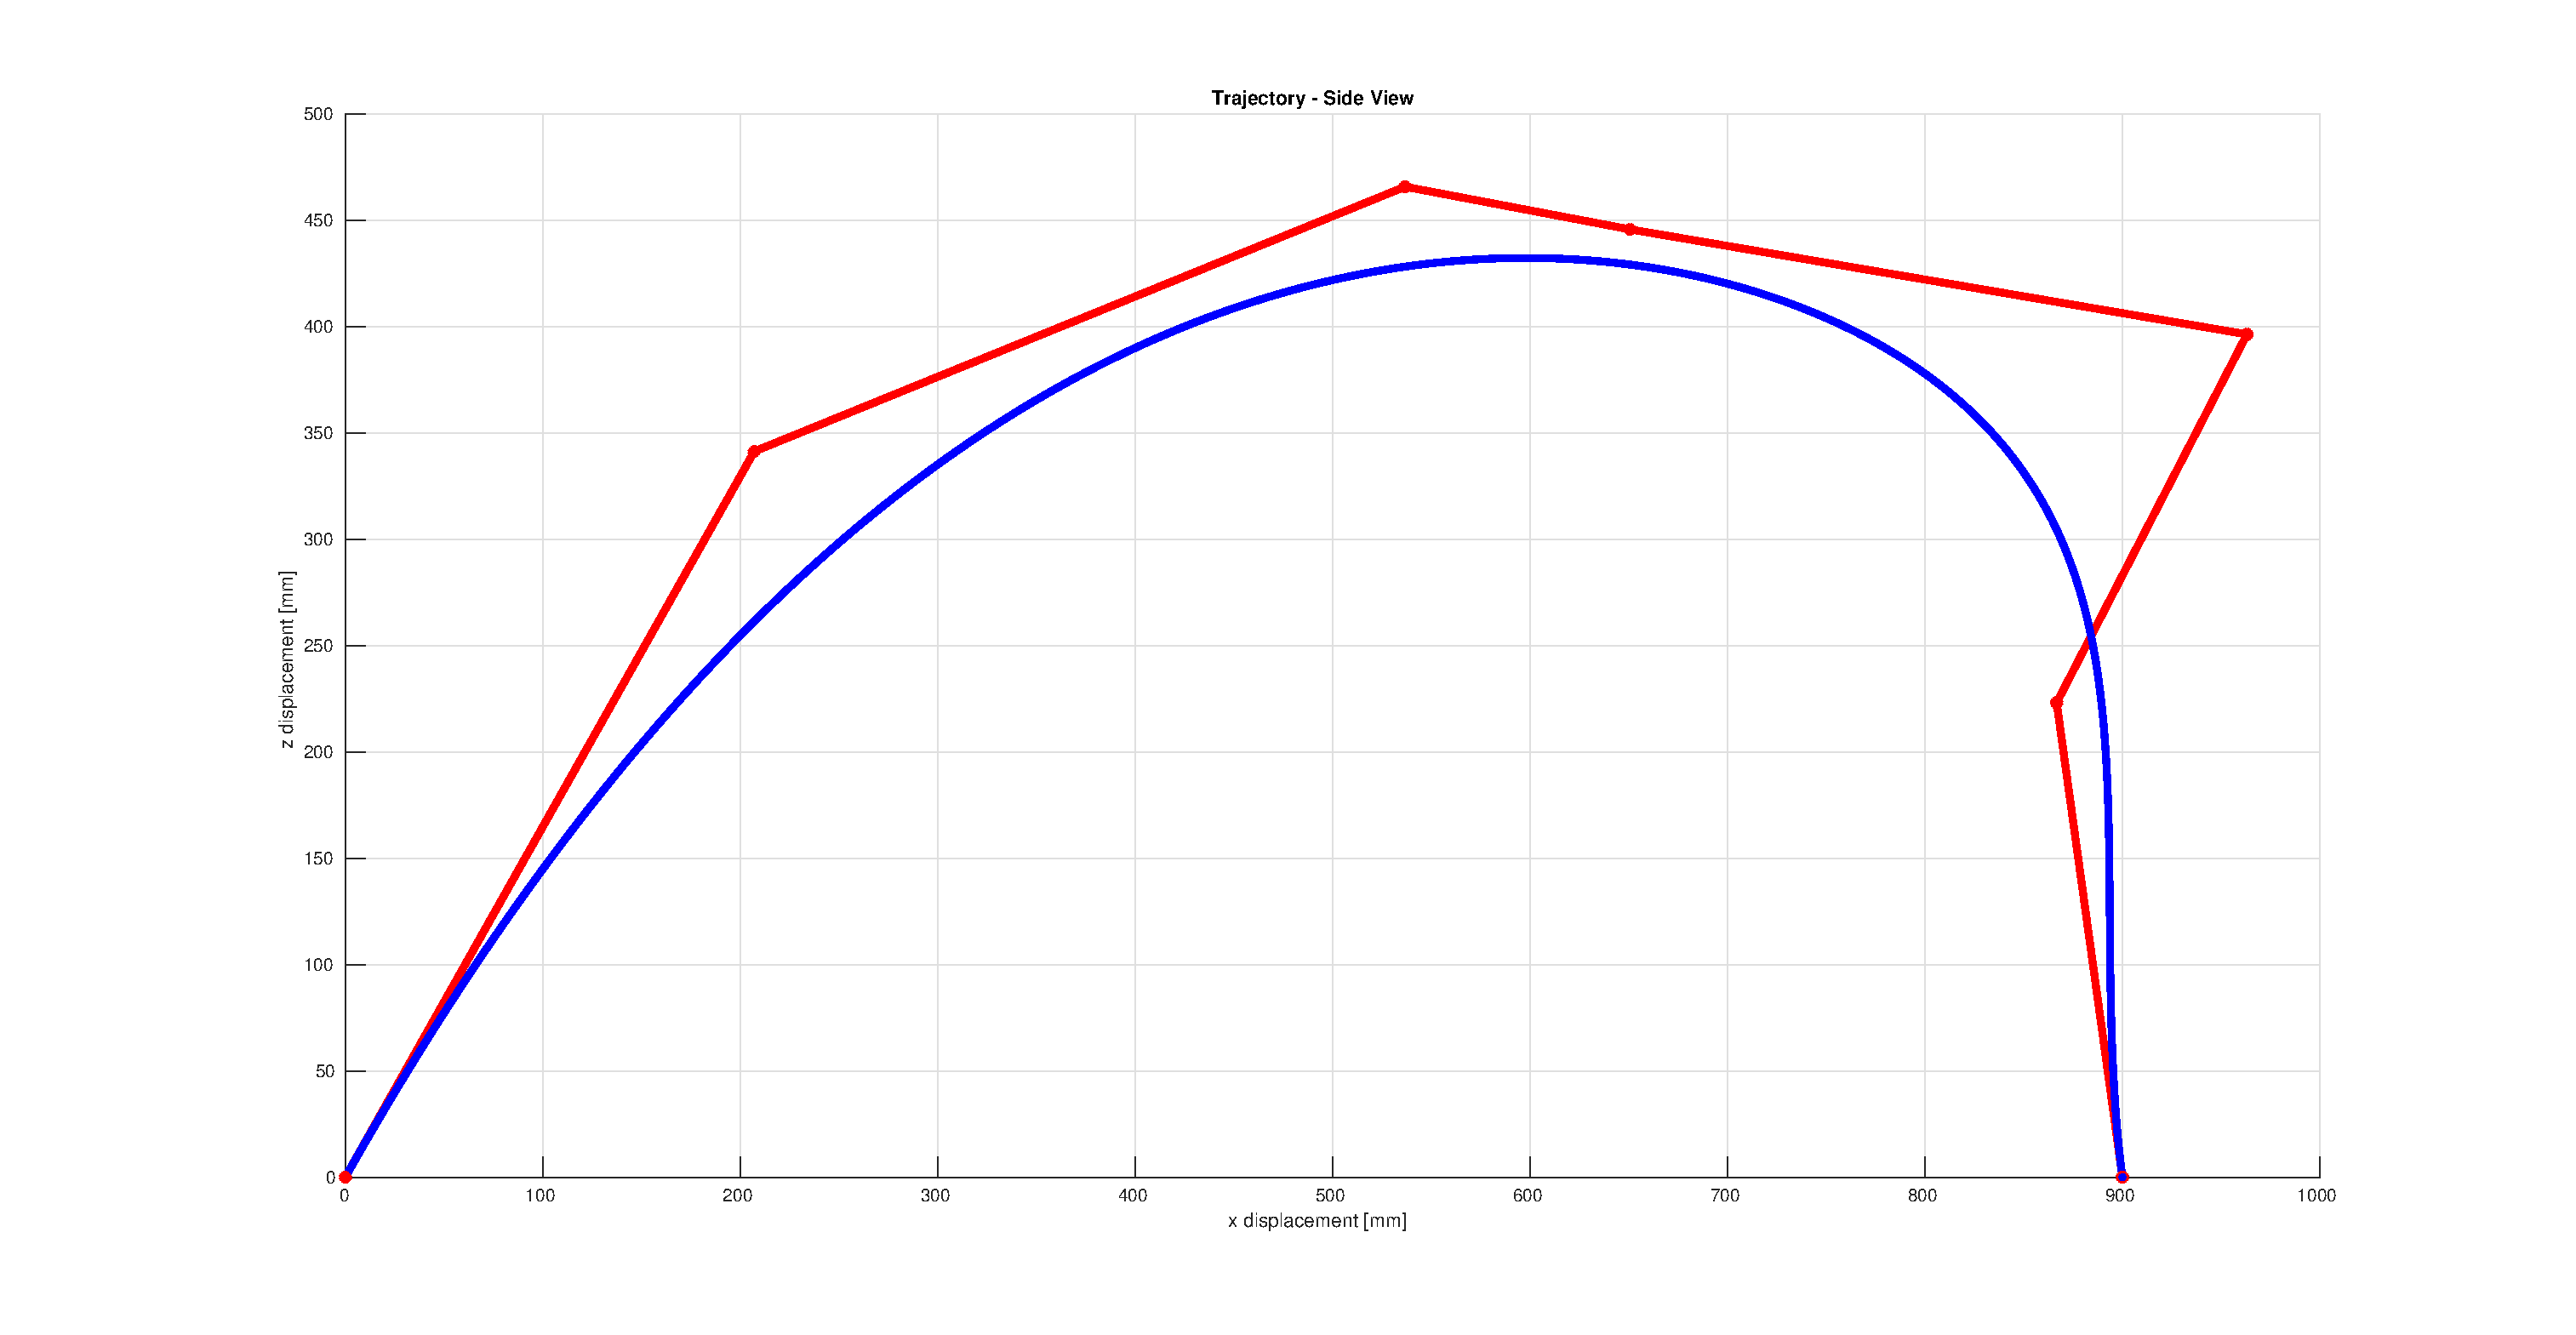
\includegraphics[height=0.45\linewidth, width=0.45\linewidth]{trajectory_simplify_no_subdivide_side.eps}
					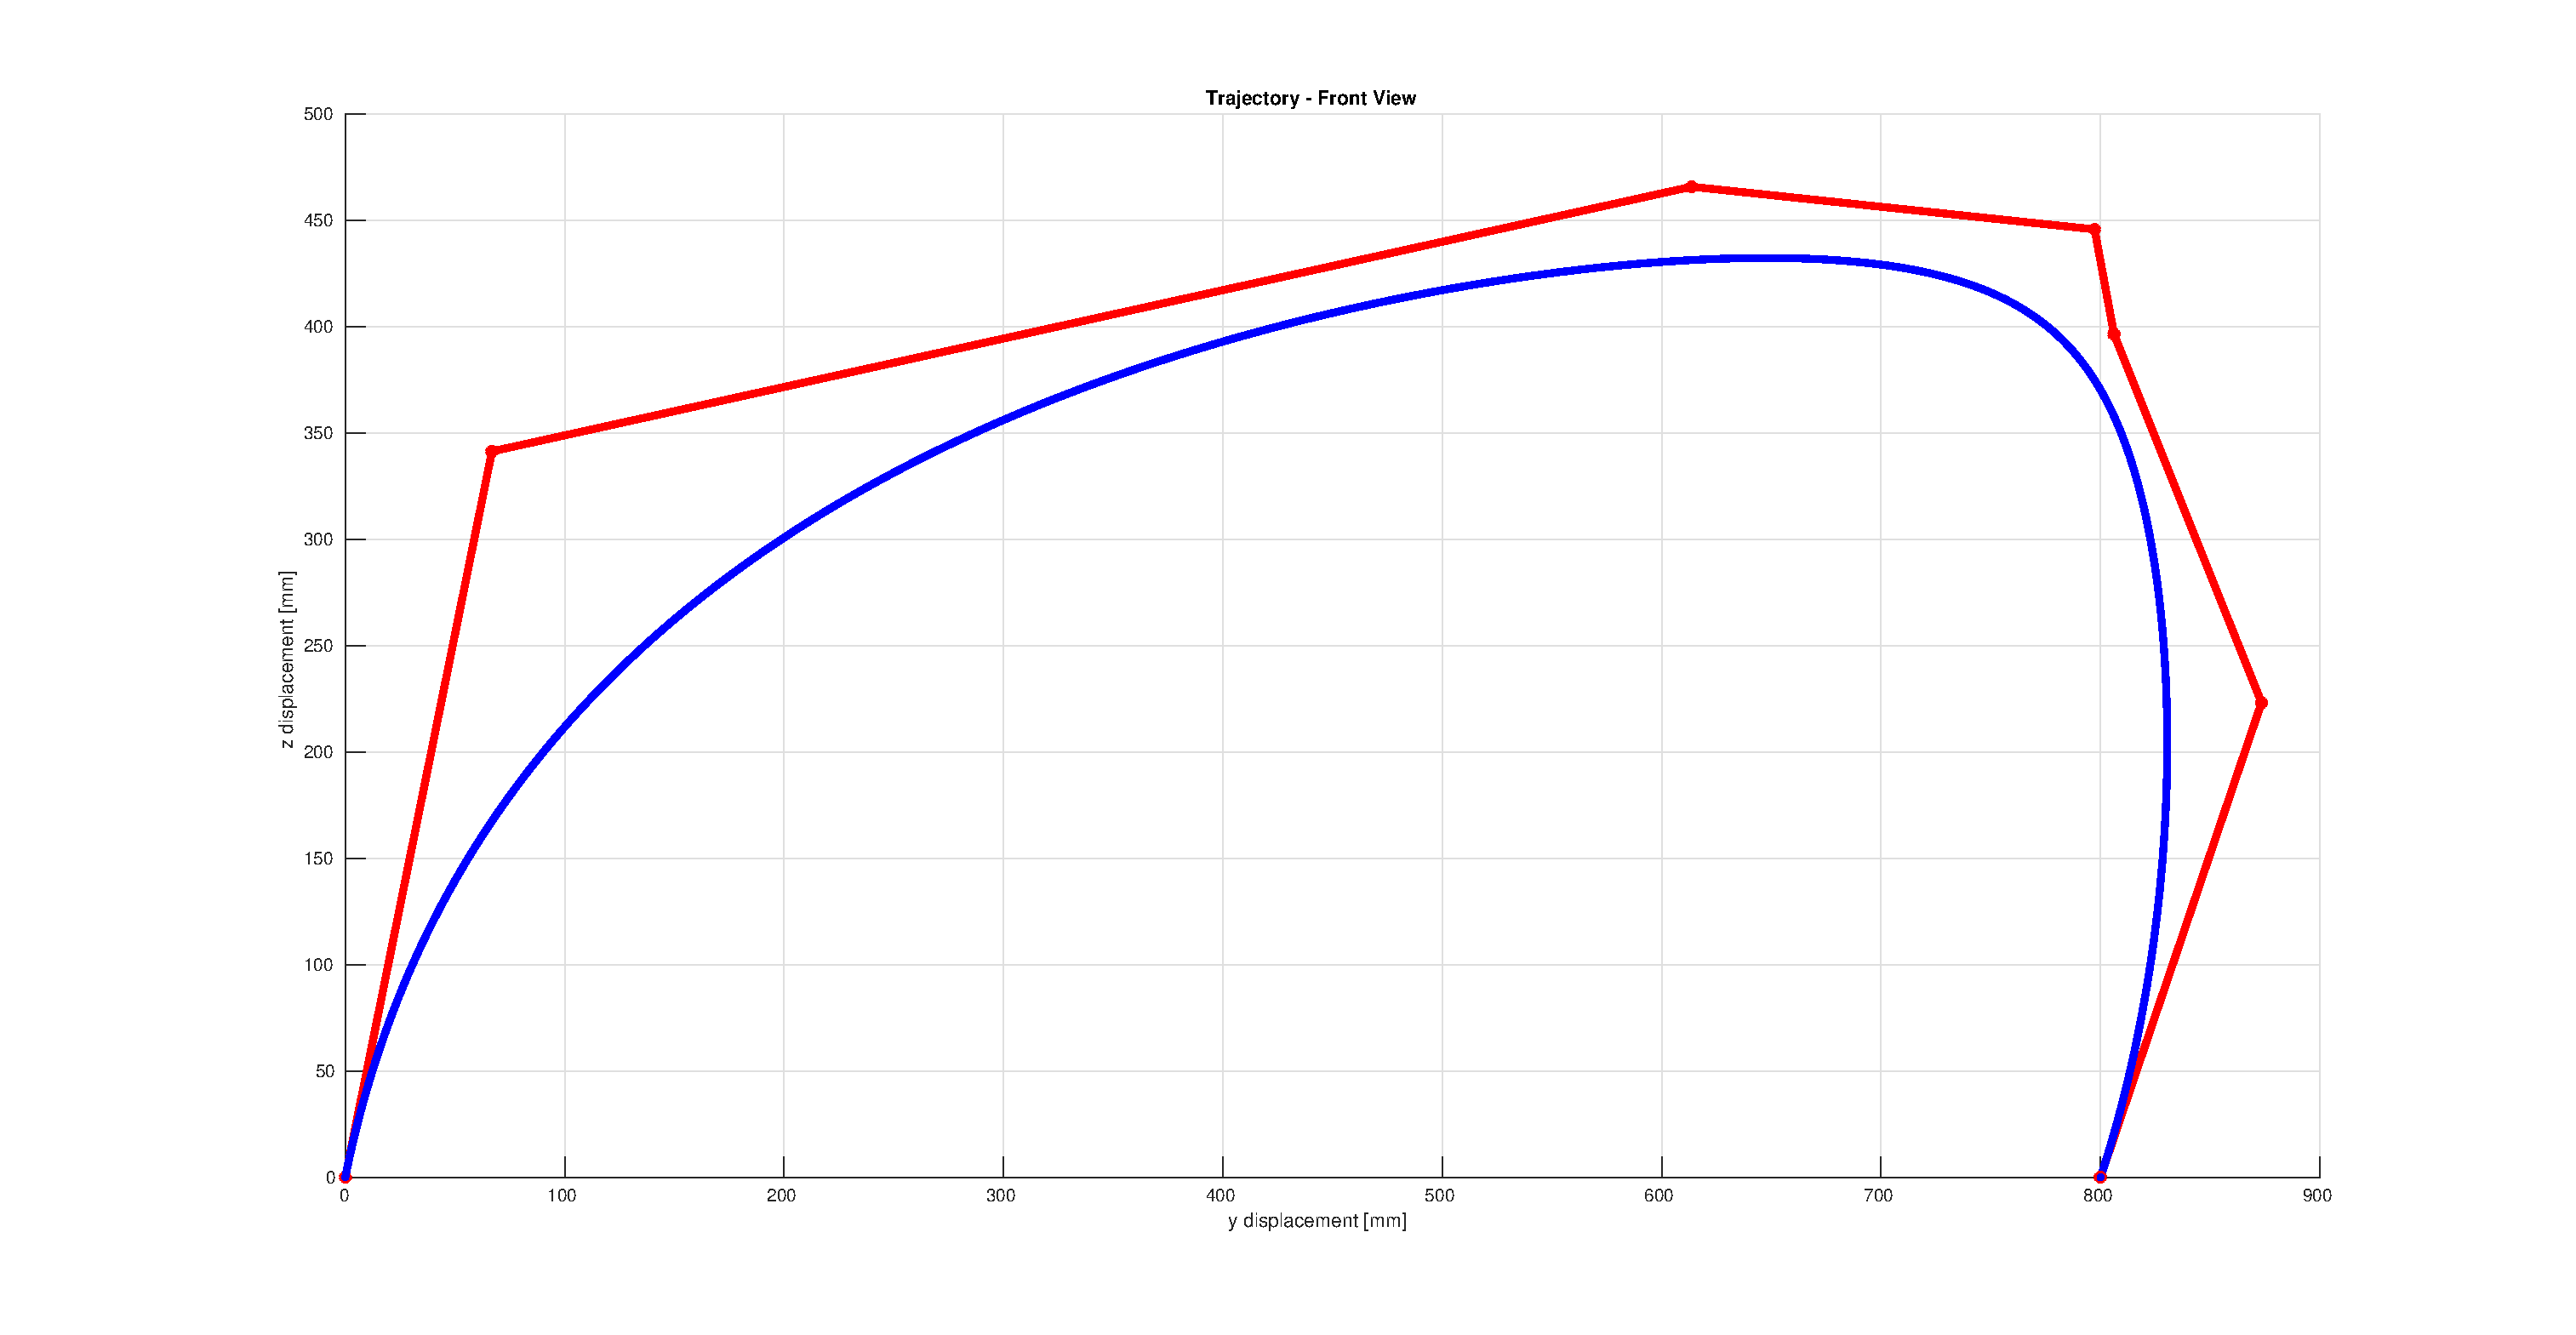
\includegraphics[height=0.45\linewidth, width=0.45\linewidth]{trajectory_simplify_no_subdivide_front.eps}
					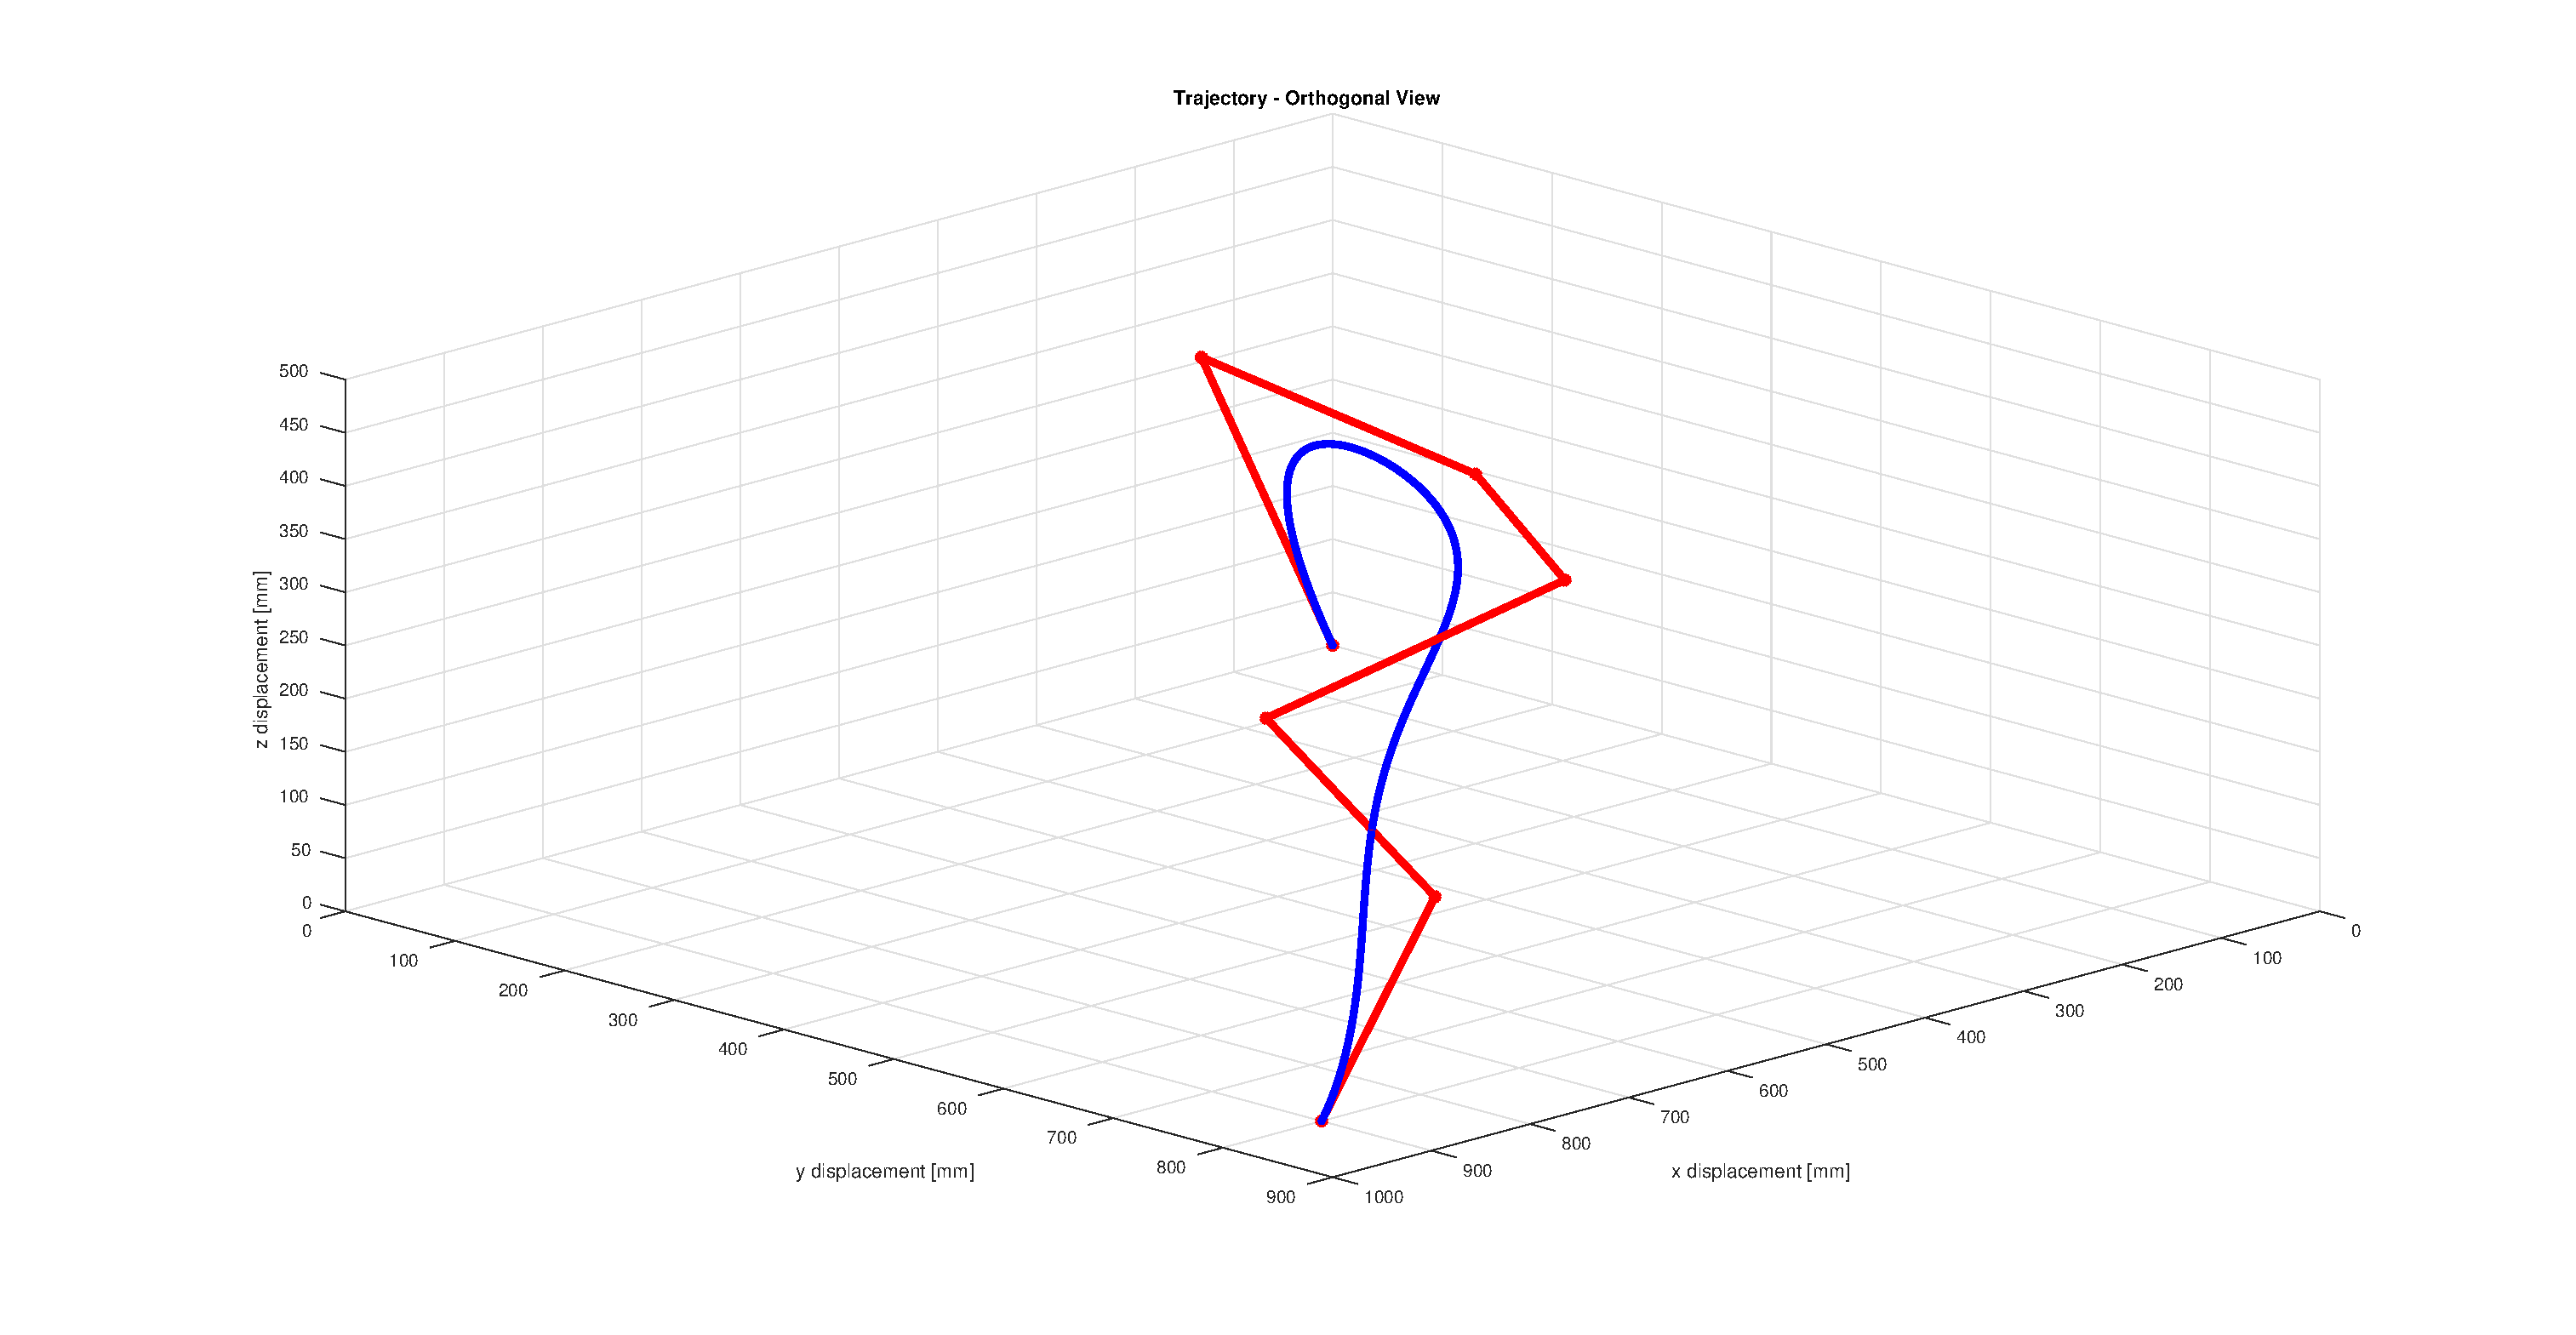
\includegraphics[height=0.45\linewidth, width=0.45\linewidth]{trajectory_simplify_no_subdivide_orthogonal.eps}
					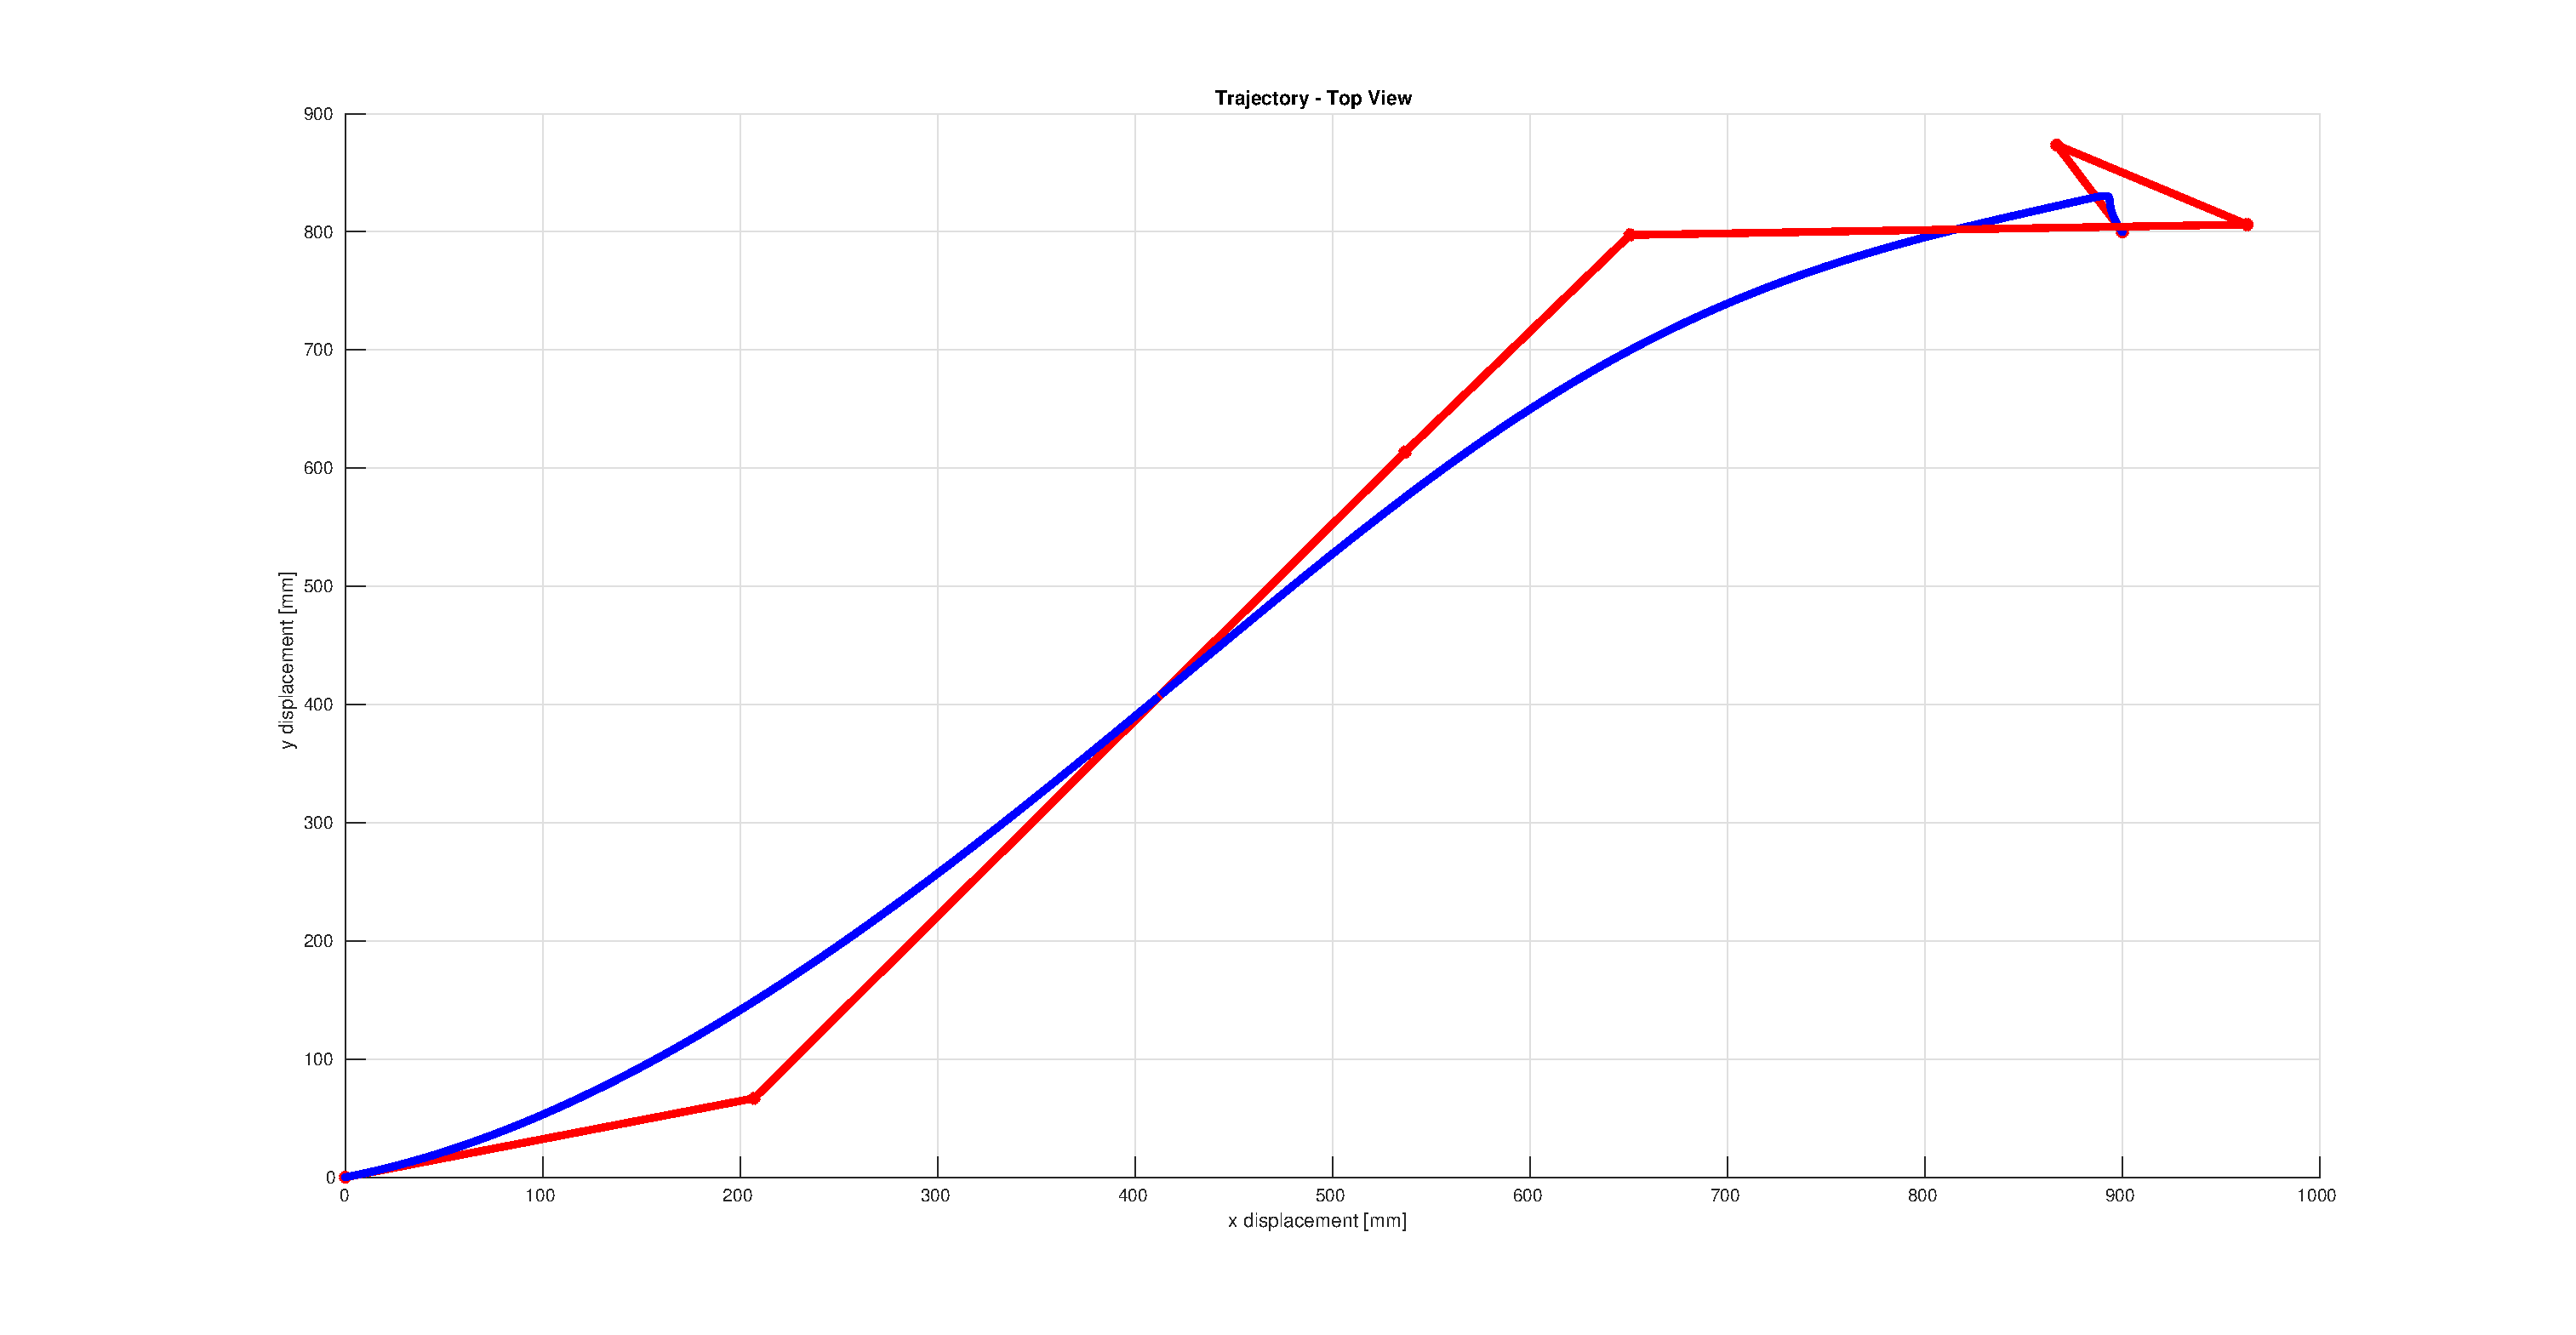
\includegraphics[height=0.45\linewidth, width=0.45\linewidth]{trajectory_simplify_no_subdivide_top.eps}
				\end{minipage}
				\caption{Sample Trajectory without Augmenting $\setofposes$}
				\label{fig:sample_trajectory_after_simplification}
			\end{figure}

		\column{0.5\textwidth}
			\begin{figure}[hb]
				\centering
				\begin{minipage}{0.8\linewidth}
					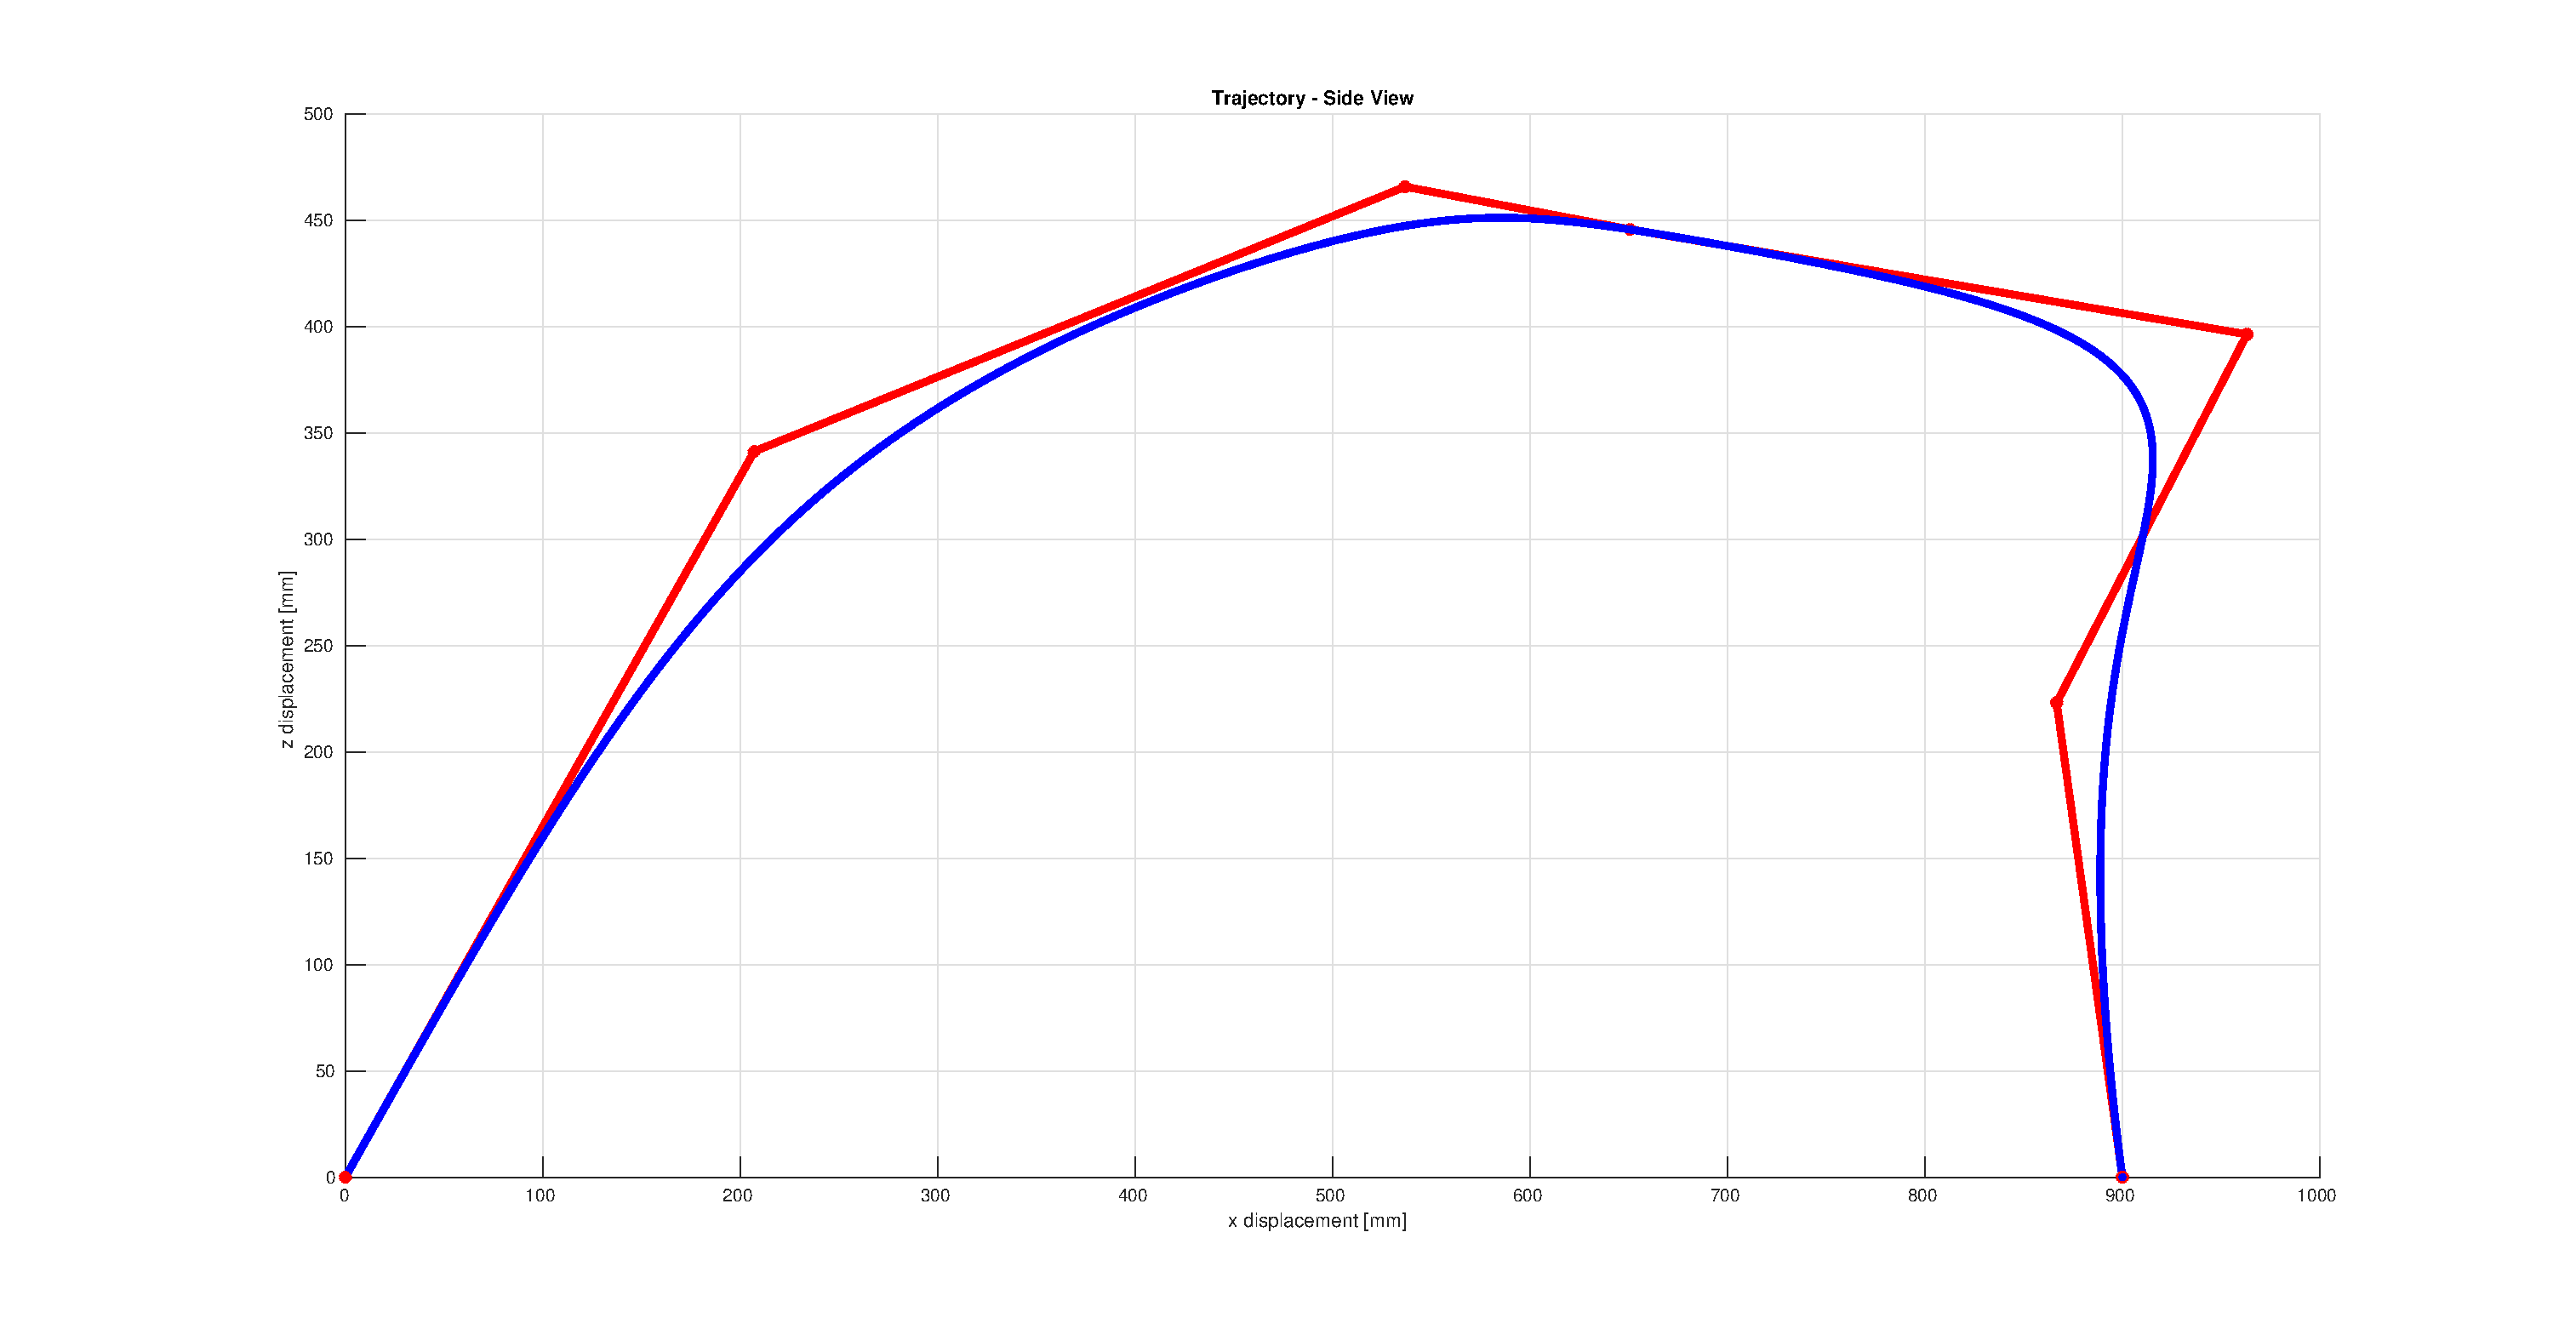
\includegraphics[height=0.45\linewidth, width=0.45\linewidth]{trajectory_simplify_subdivide_side.eps}
					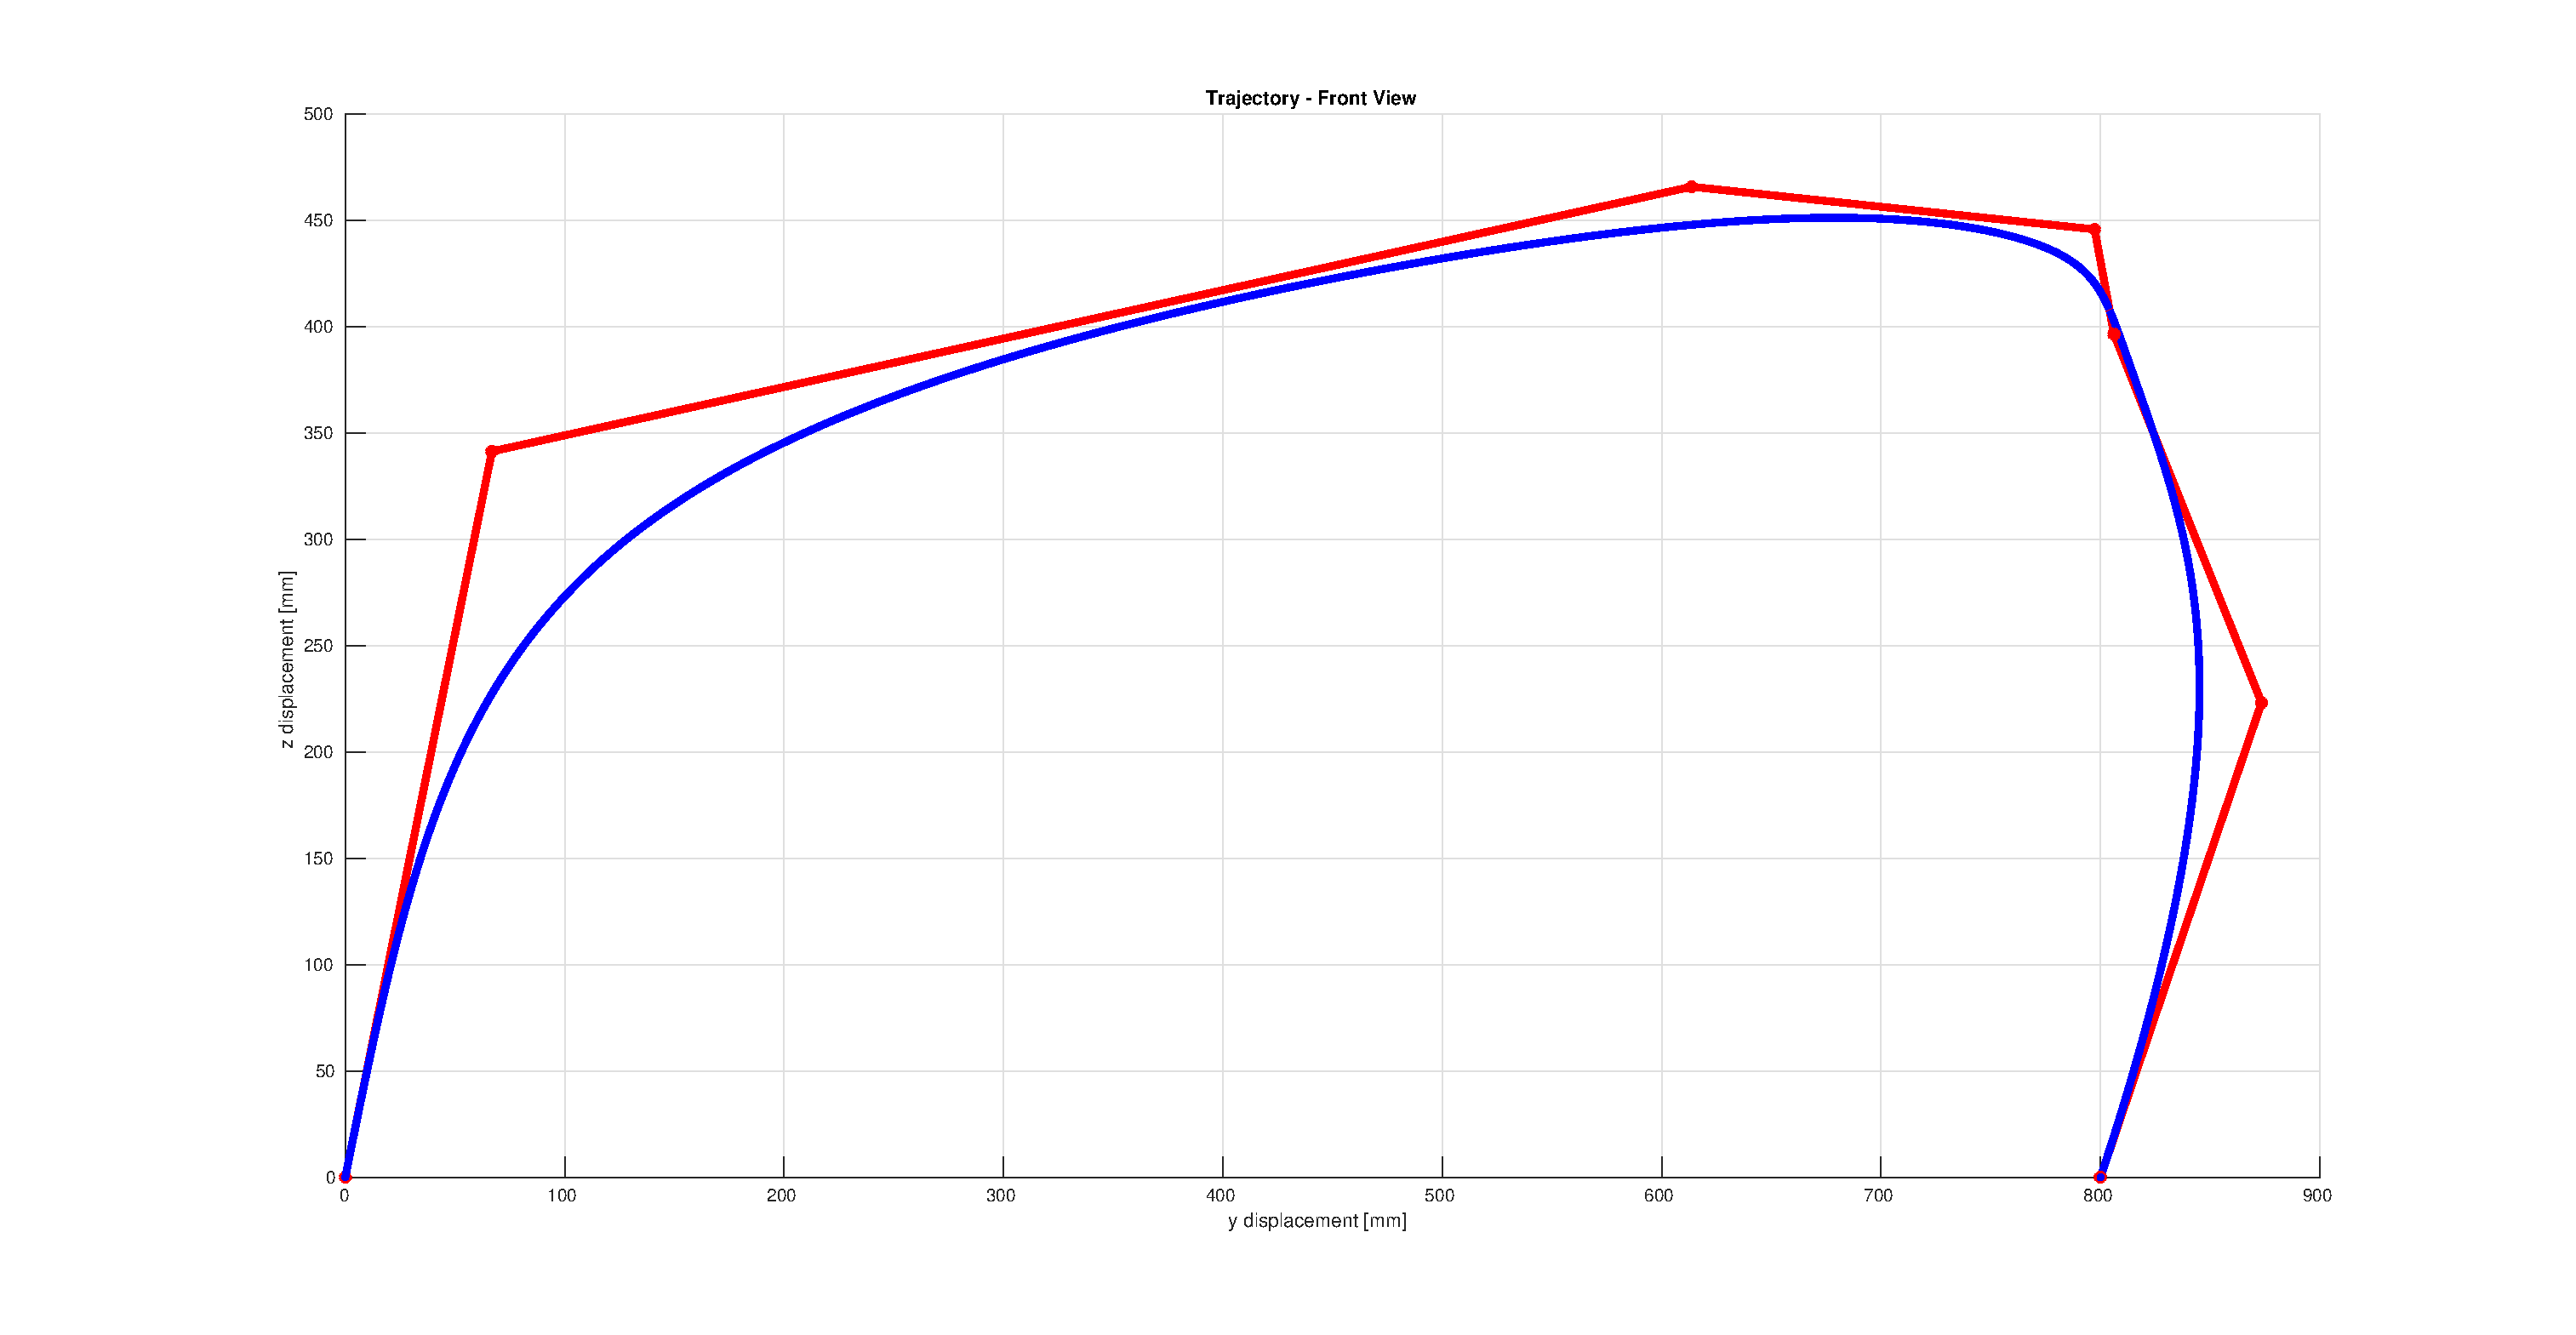
\includegraphics[height=0.45\linewidth, width=0.45\linewidth]{trajectory_simplify_subdivide_front.eps}
					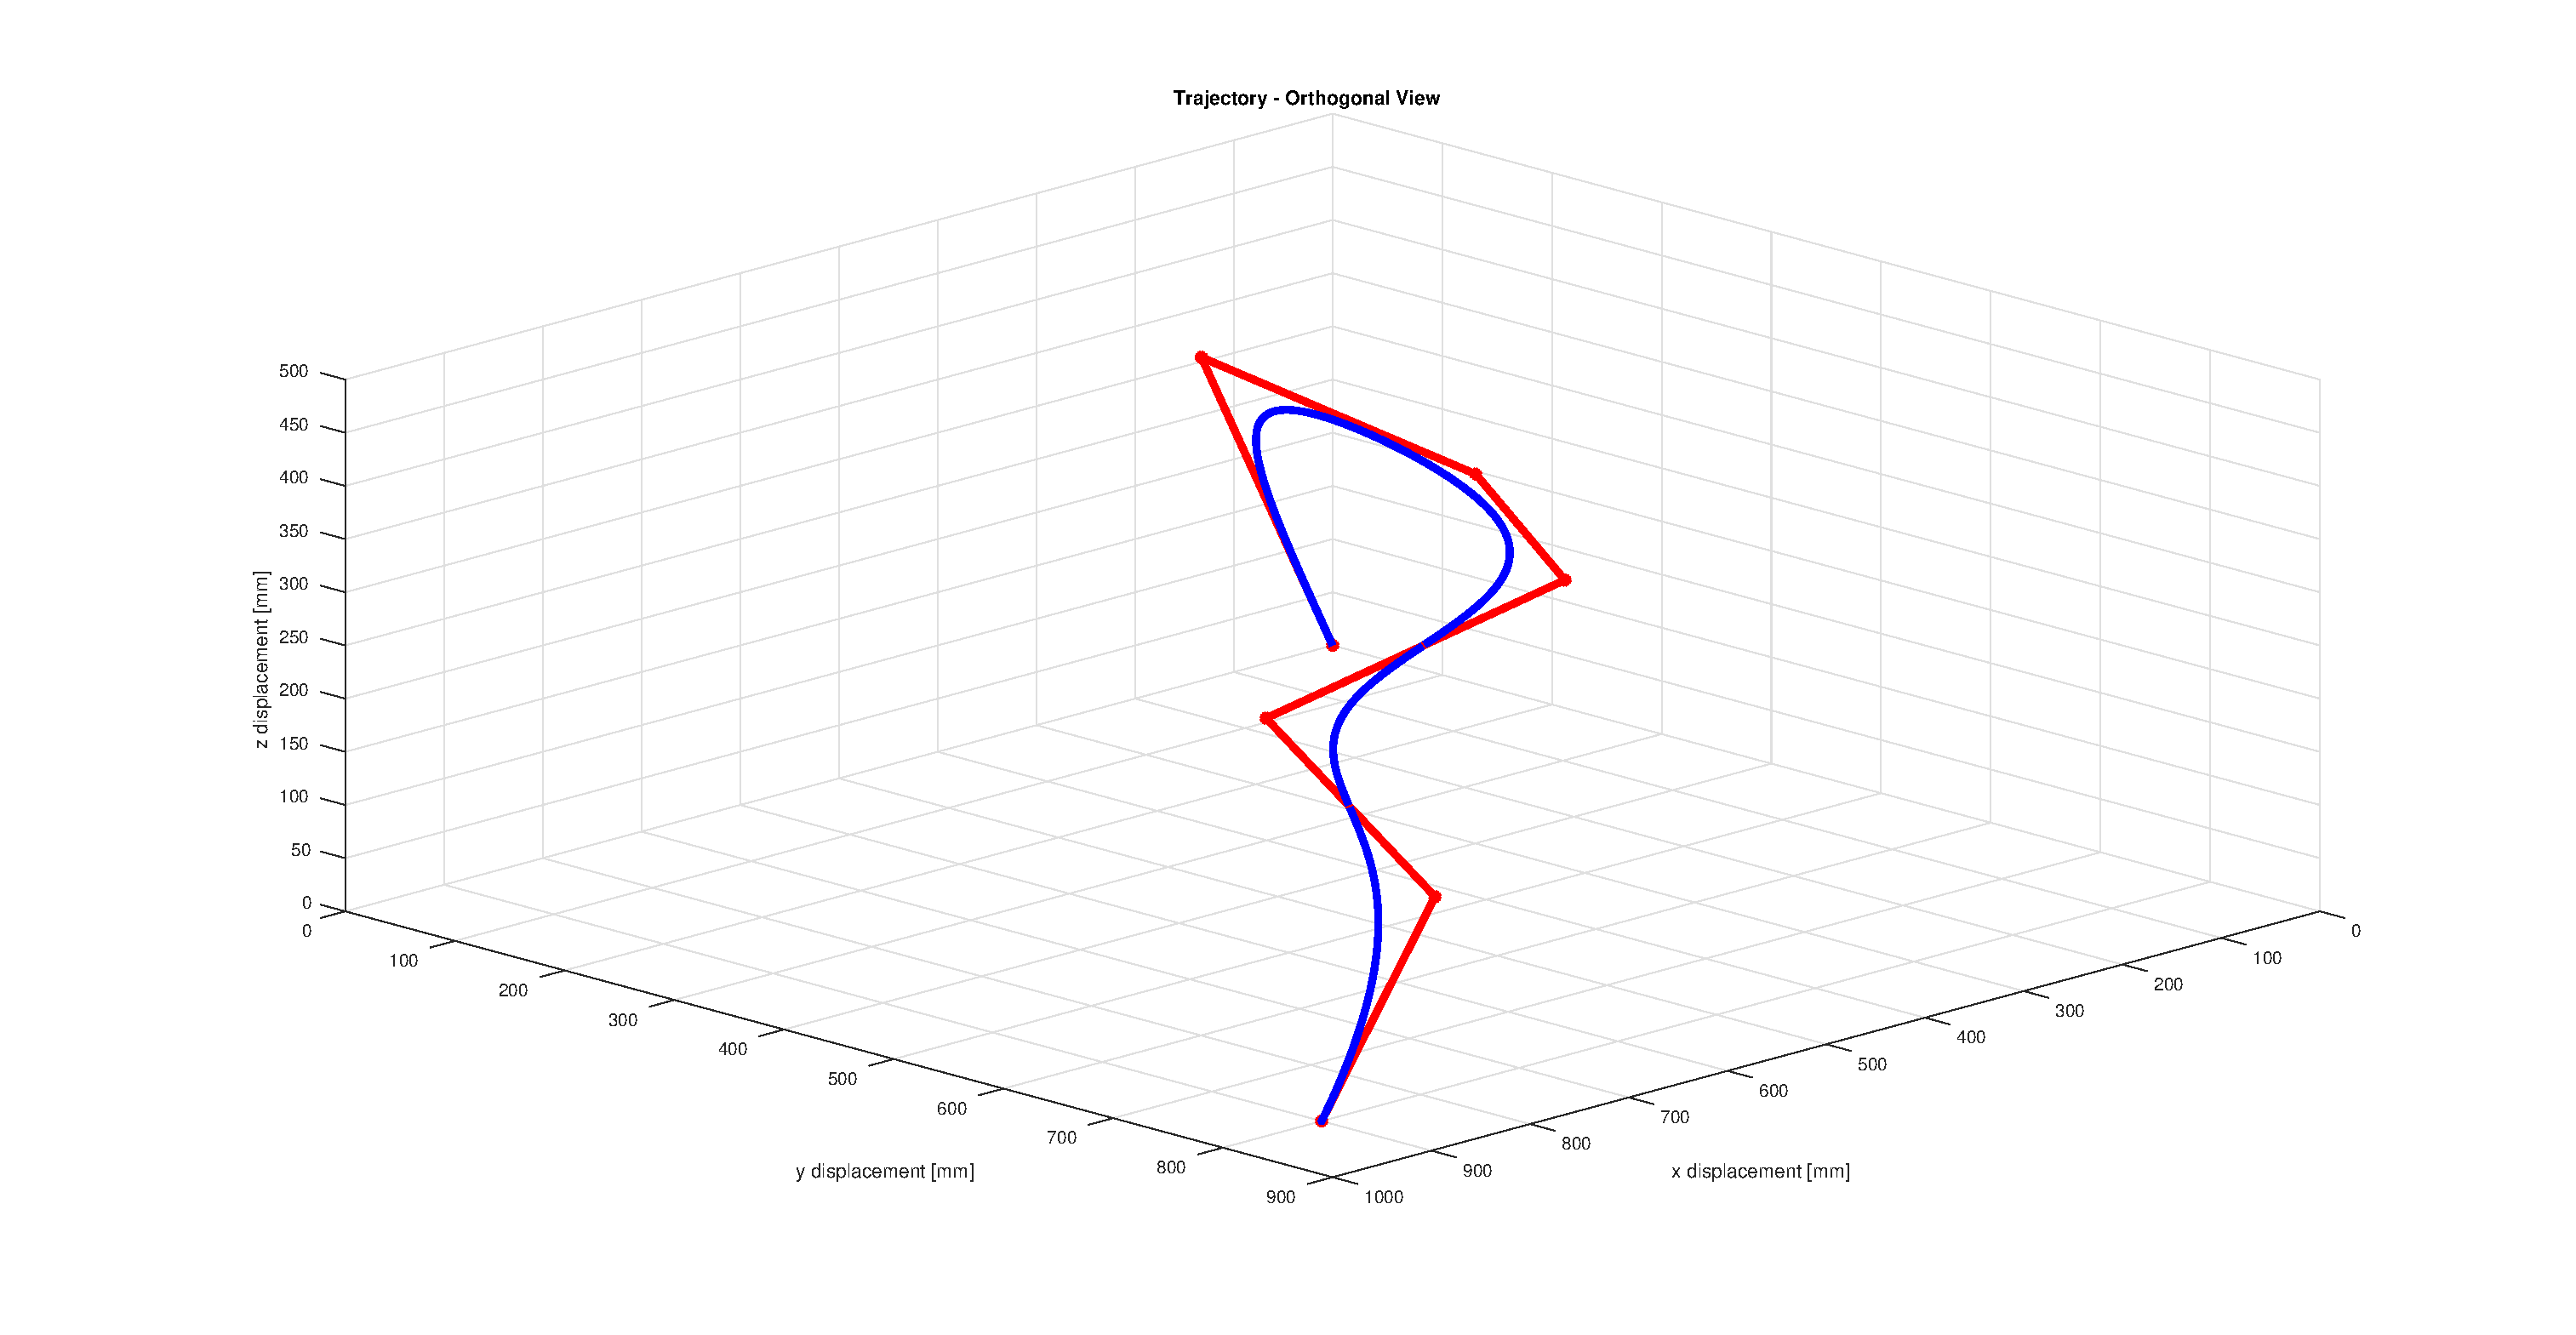
\includegraphics[height=0.45\linewidth, width=0.45\linewidth]{trajectory_simplify_subdivide_orthogonal.eps}
					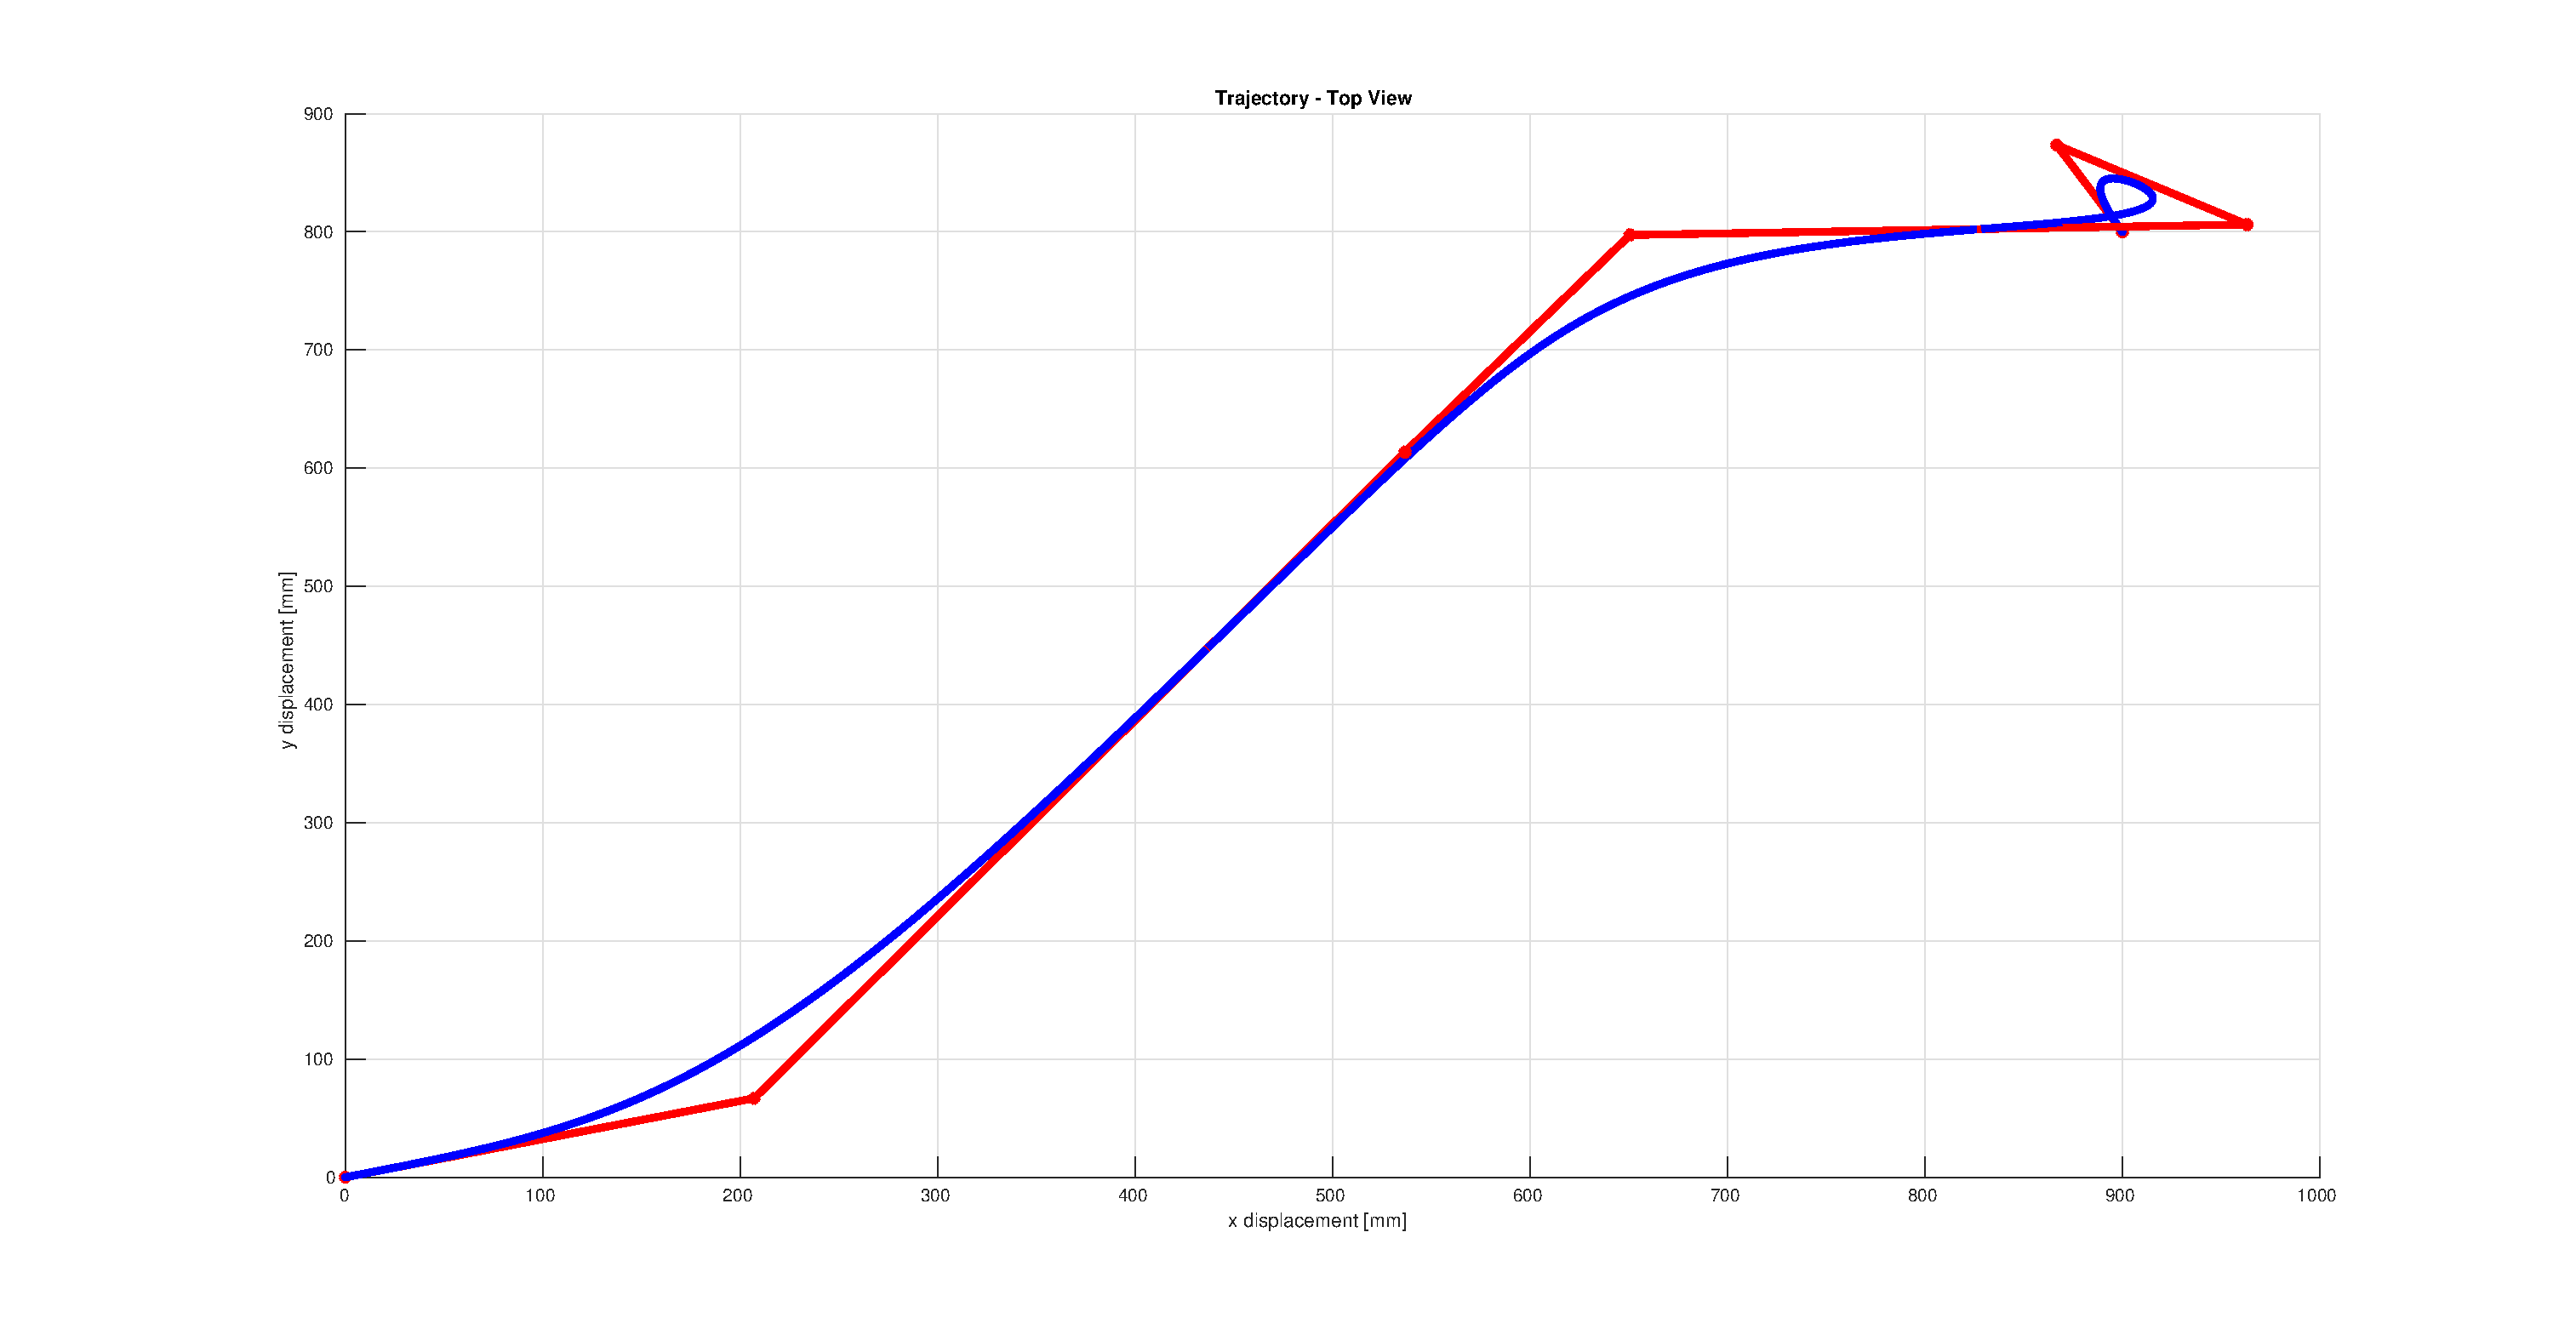
\includegraphics[height=0.45\linewidth, width=0.45\linewidth]{trajectory_simplify_subdivide_top.eps}
				\end{minipage}
				\caption{Sample Trajectory with Augmented $\setofposes$}
				\label{fig:sample_trajectory_with_augmented_set_of_poses}
			\end{figure}
	\end{columns}
\end{frame}

\begin{frame}
	\frametitle{Path-Planning Demo}

	\movie[
		height = 5cm,
		width = 5cm,
		externalviewer,
		showcontrols
	]
	{Demo}{./demos/demos/complex_rotation_avoid.mp4}
\end{frame}

\begin{frame}
	\frametitle{Motion Law}

	\begin{figure}[hb]
		\centering
		\def\svgwidth{0.5\textwidth}
		\import{res/img/}{motion_law_intuition.pdf_tex}
		\caption{Motion Law Construction}%
		\label{fig:motion_law_graphical_intuition}
	\end{figure}

\end{frame}

\begin{frame}
	\frametitle{Motion Law Output}
	\begin{figure}[hb]
		\centering
		\begin{minipage}{0.45\textwidth}
			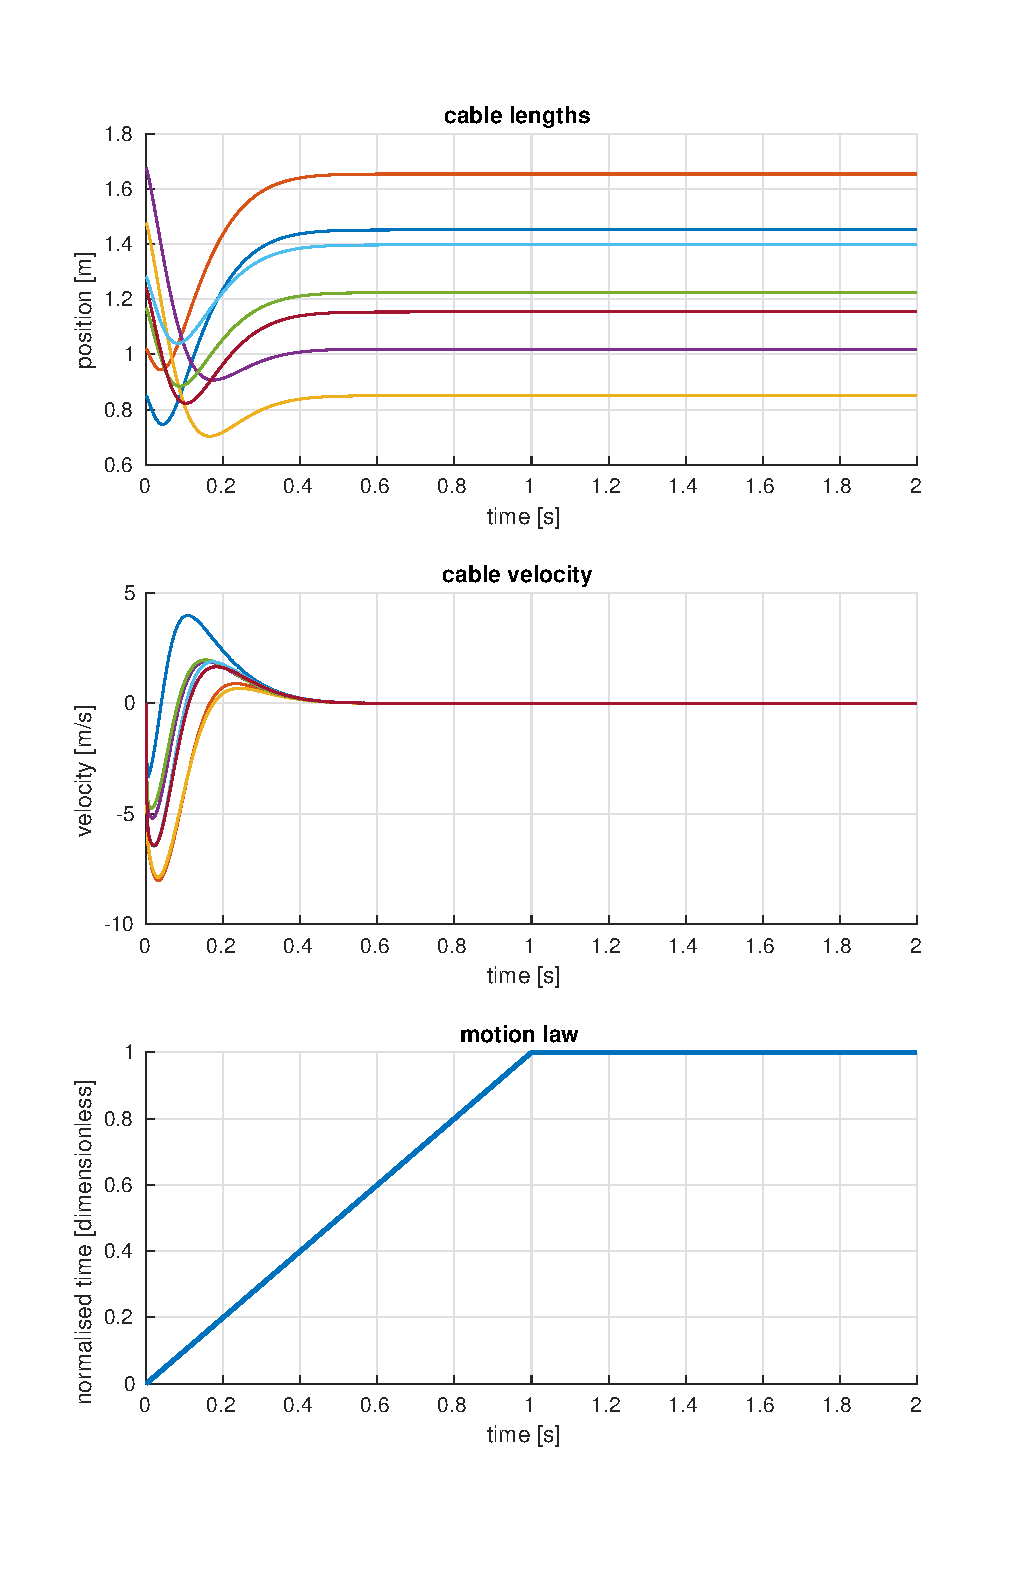
\includegraphics[width=\textwidth]{motion_law_linear}
		\end{minipage}%
		\begin{minipage}{0.45\textwidth}
			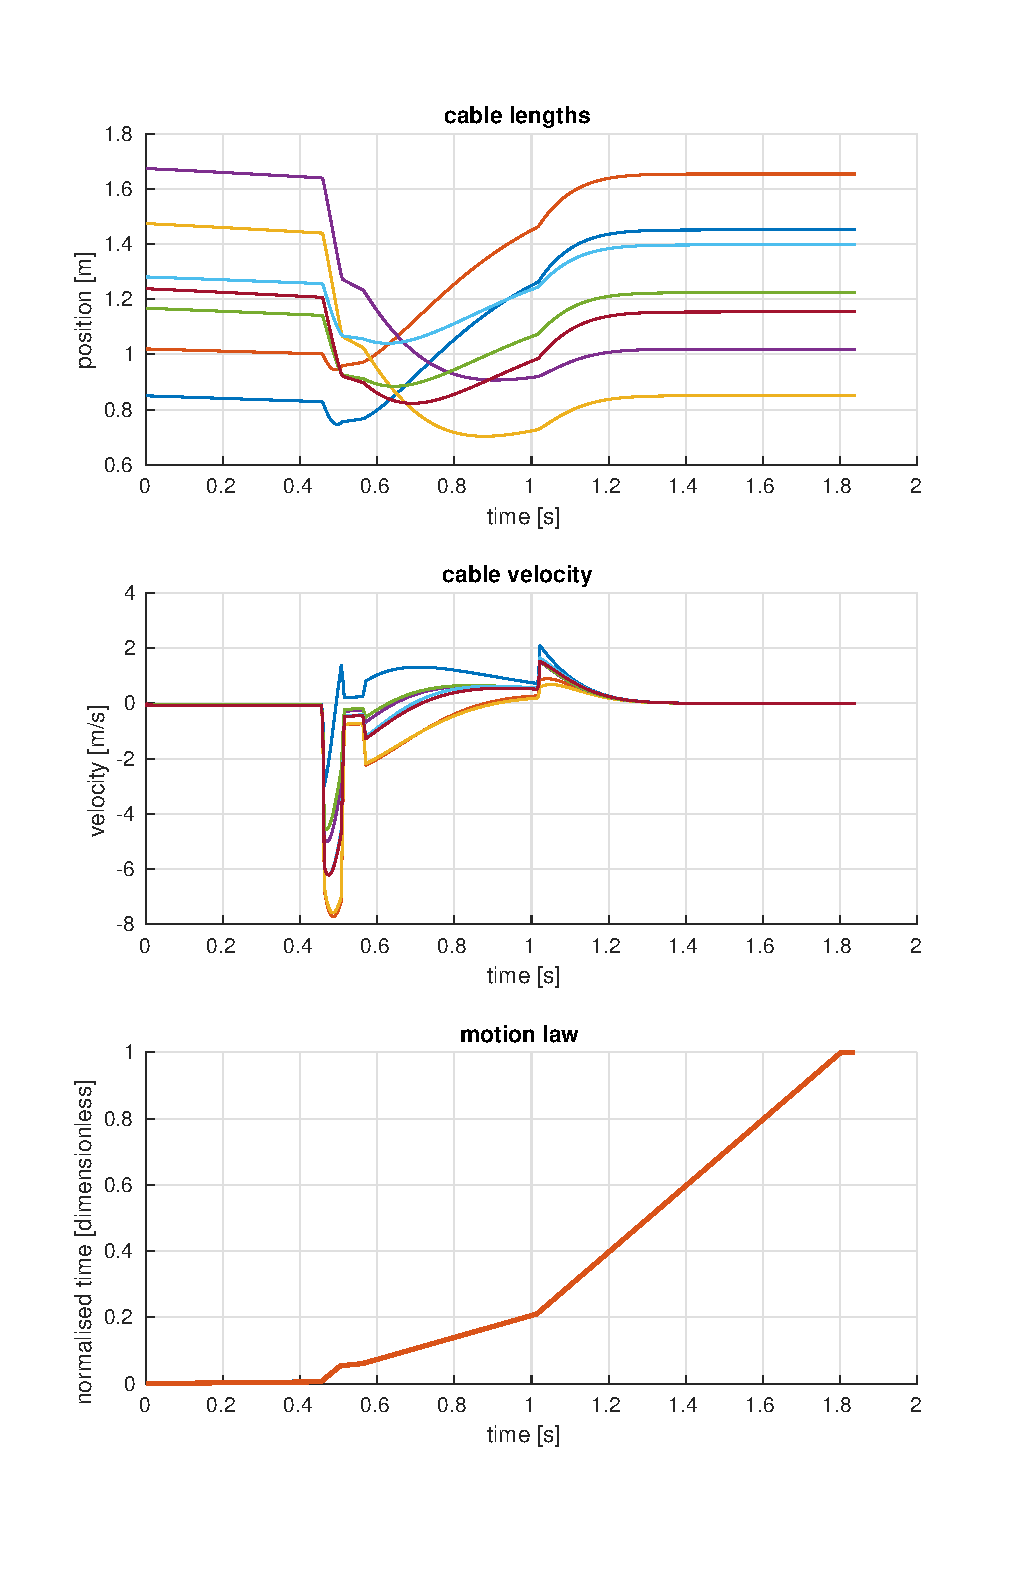
\includegraphics[width=\textwidth]{motion_law_deg_1}
		\end{minipage}
		\caption{No Motion Law (left) and Degree 1 (right) Motion Law}
		\label{fig:motion_law_lin_1}
	\end{figure}
\end{frame}
\begin{frame}
	\frametitle{Motion Law Output}

	\begin{figure}[hb]
		\centering
		\begin{minipage}{0.45\textwidth}
			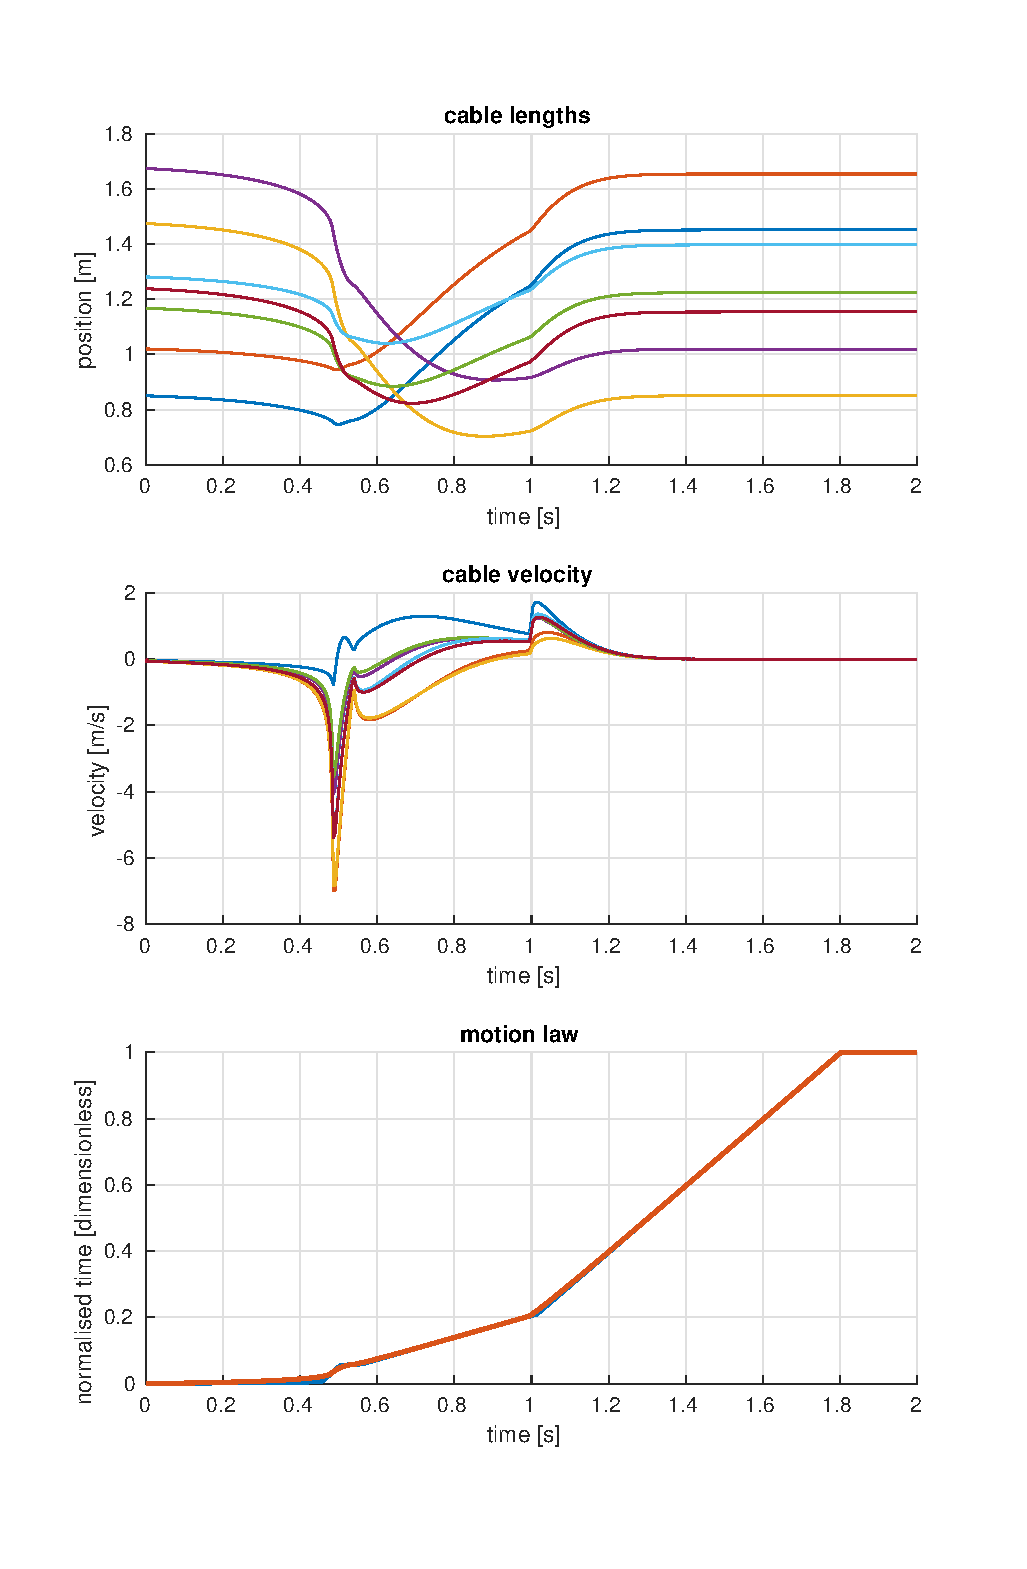
\includegraphics[width=\textwidth]{motion_law_deg_2}
		\end{minipage}%
		\begin{minipage}{0.45\textwidth}
			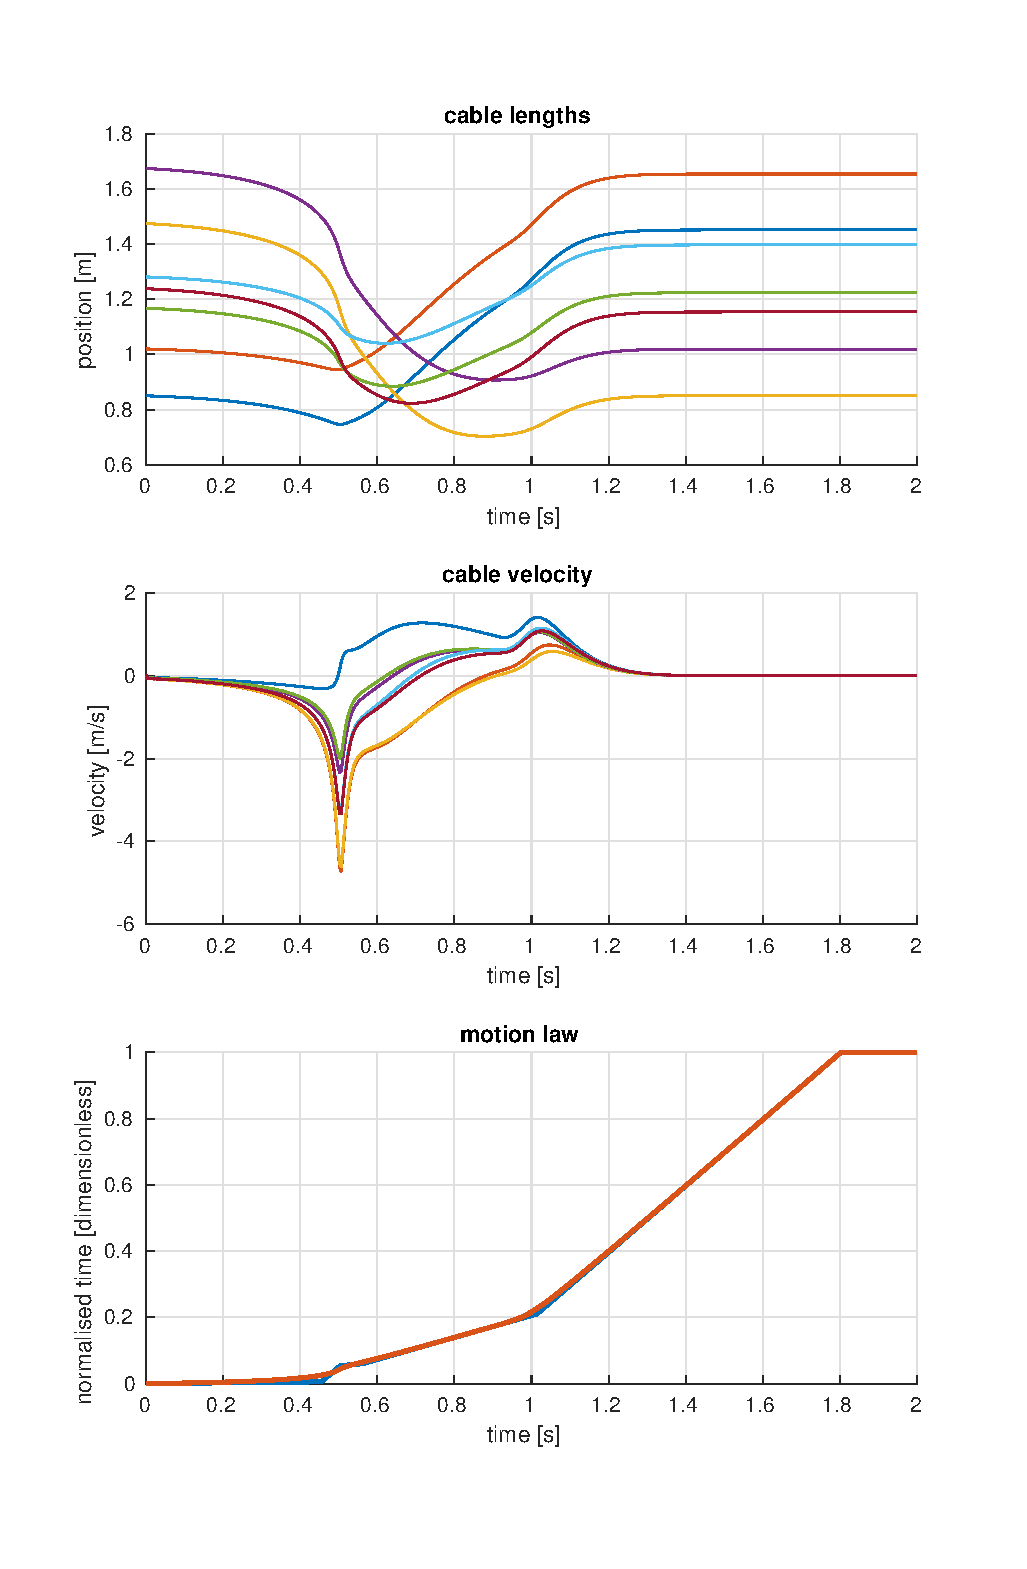
\includegraphics[width=\textwidth]{motion_law_deg_3}
		\end{minipage}%
		\caption{Degree 2 (left) and Degree 3 (right) Motion Law}
		\label{fig:motion_law_2_3}
	\end{figure}
\end{frame}

\begin{frame}
	\frametitle{Motion Law Output}

	\begin{figure}[hb]
		\centering
		\begin{minipage}{0.45\textwidth}
			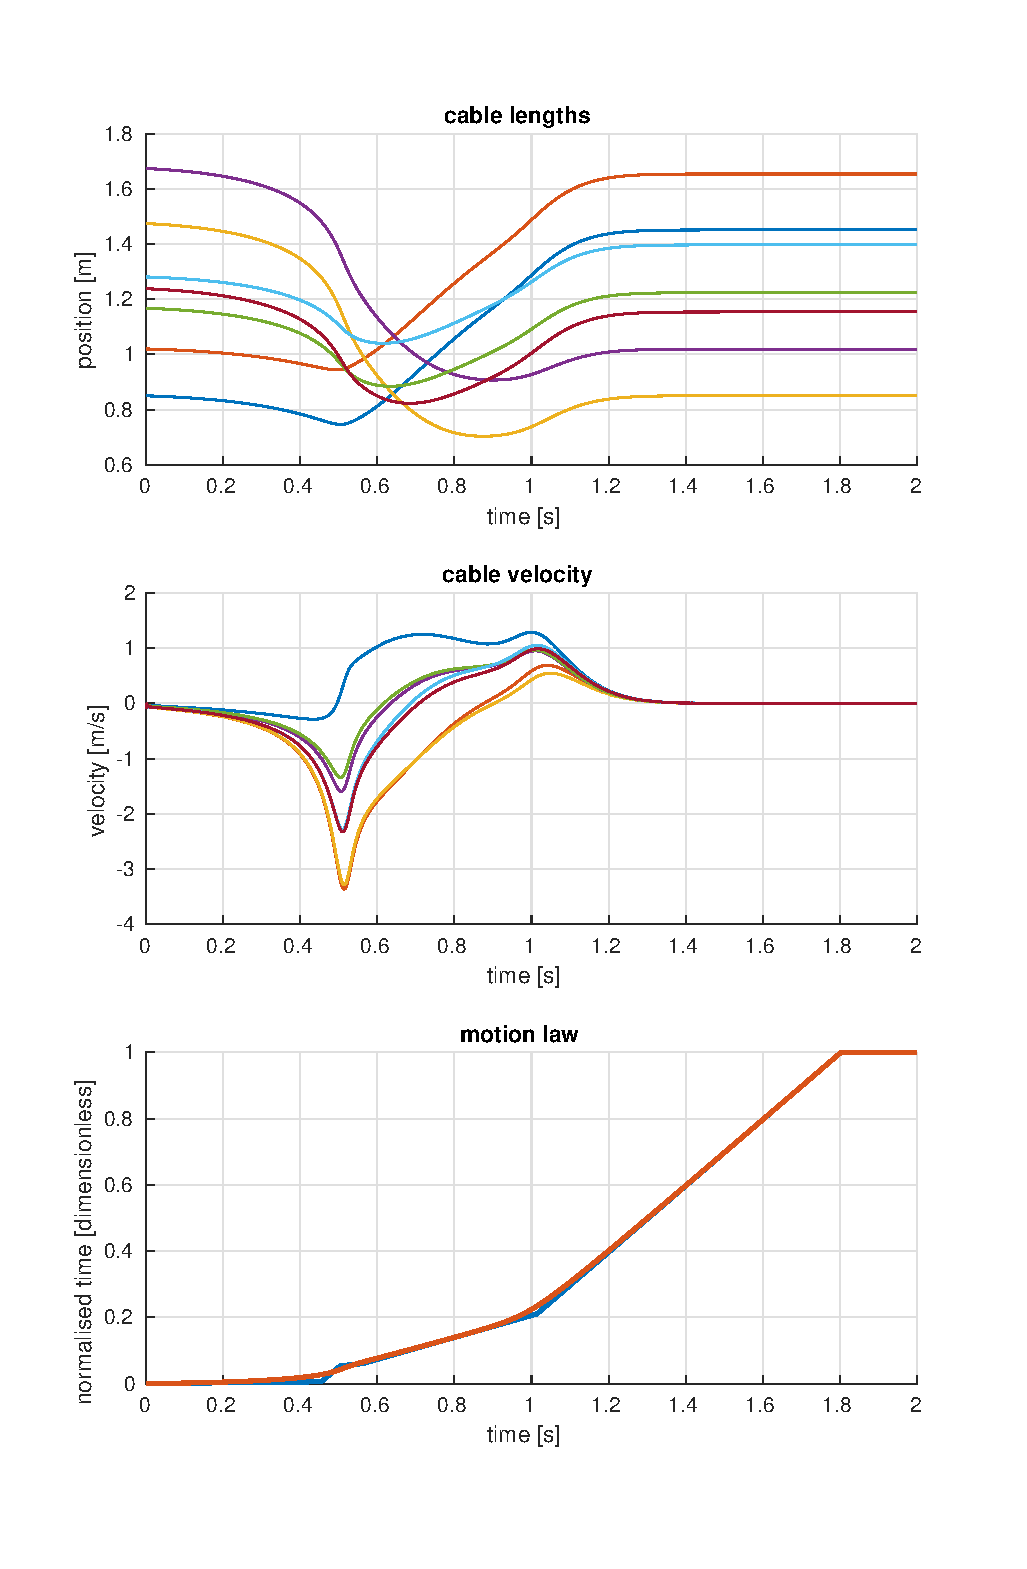
\includegraphics[width=\textwidth]{motion_law_deg_4}
		\end{minipage}%
		\begin{minipage}{0.45\textwidth}
			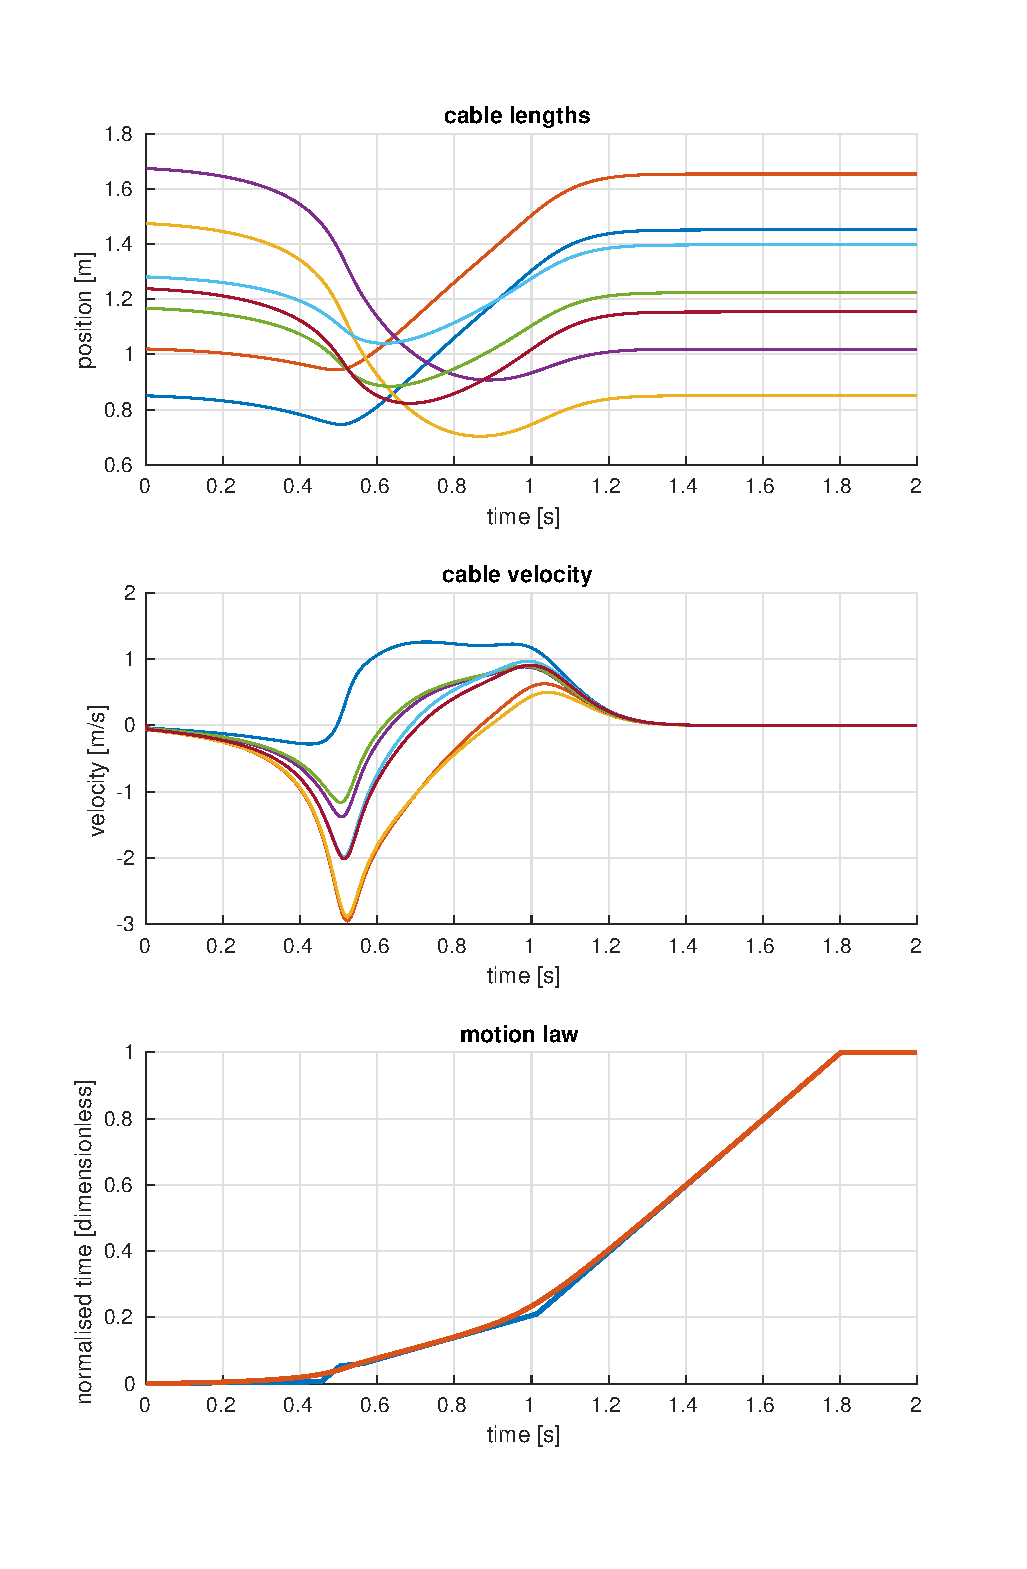
\includegraphics[width=\textwidth]{motion_law_deg_5}
		\end{minipage}%
		\caption{Degree 4 (left) and Degree 5 (right) Motion Law}
		\label{fig:motion_law_4_5}
	\end{figure}
\end{frame}

\begin{frame}
	\frametitle{Motion Law Output}

	\begin{figure}[hb]
		\centering
		\begin{minipage}{0.45\textwidth}
			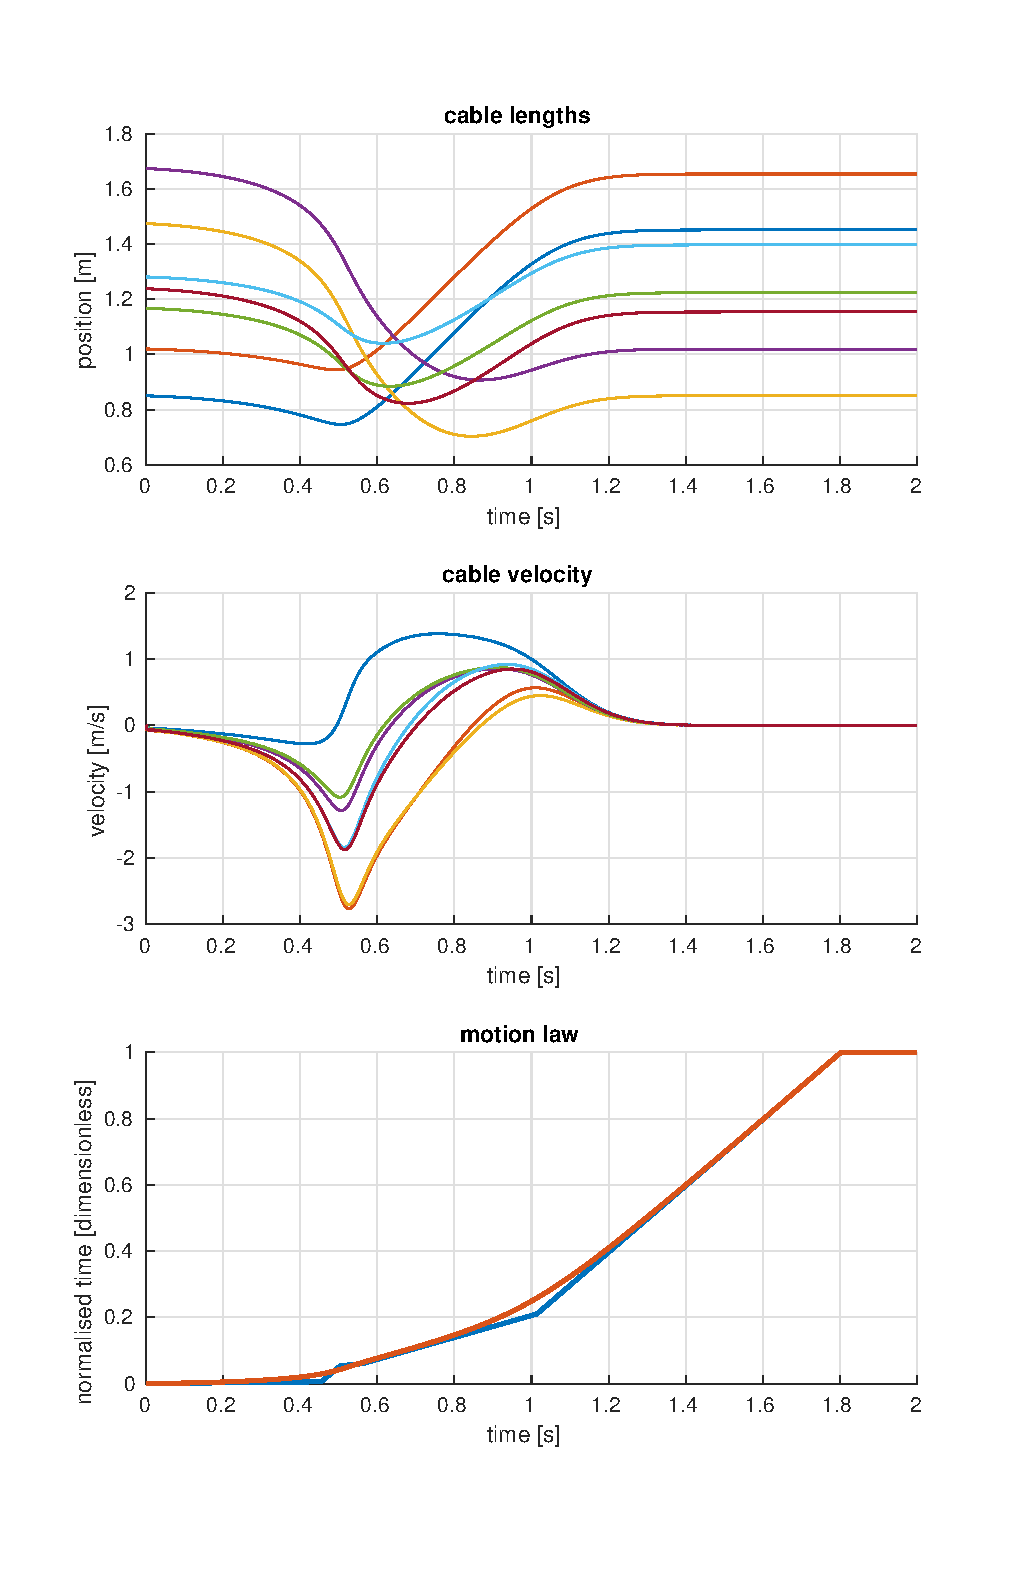
\includegraphics[width=\textwidth]{motion_law_deg_6}
		\end{minipage}%
		\begin{minipage}{0.45\textwidth}
			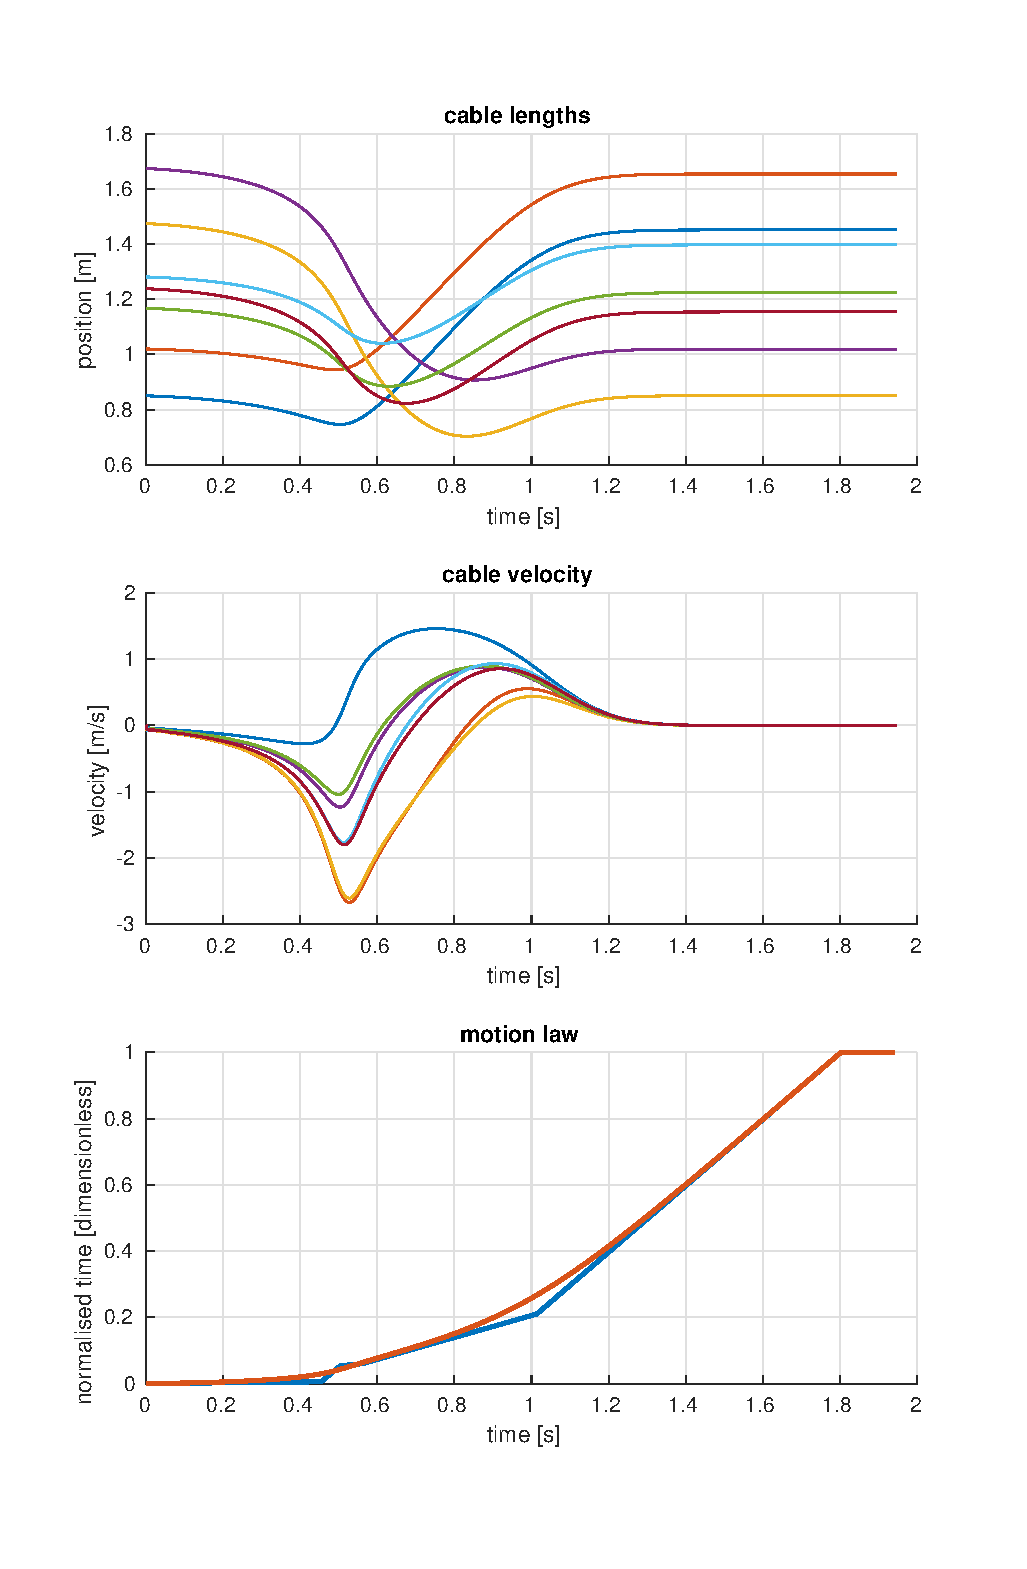
\includegraphics[width=\textwidth]{motion_law_deg_7}
		\end{minipage}%
		\caption{Degree 6 (left) and Degree 7 (right) Motion Law}
		\label{fig:motion_law_6_7}
	\end{figure}
\end{frame}

	\section{Conclusion}
		\begin{frame}
	\frametitle{Conclusion}

	\begin{itemize}
		
		\item

			Used RRT-based algorithm for path planning

		\item

			Incorporated capacity margin step in the algorithm

		\item

			Developed various post-processing techniques to simplify path

		\item

			Proposed distance measure that can be used for planning with CDPRs

		\item

			Use B-splines to guarantee high degree of smoothness

		\item

			Developed method to guarantee B-splines are free of collisions

	\end{itemize}
\end{frame}


	\begin{frame}
		\frametitle{Bibliography}
		\printbibliography{}
	\end{frame}
\end{document}
